\documentclass[12pt]{article}
\usepackage{amsthm}
\usepackage{bbm}
\usepackage{amssymb}
\usepackage{mathtools}
\mathtoolsset{showonlyrefs,showmanualtags}
\usepackage{etoolbox}
% \usepackage{booktabs}
% \usepackage{url}
\usepackage{setspace}
\usepackage[margin=1in]{geometry}
\usepackage{authblk}
\usepackage{natbib}
% \usepackage[page]{appendix}
% \usepackage[nomarkers,nolists]{endfloat}
\usepackage{graphicx}
% \usepackage{caption}
% \usepackage{subcaption}
\usepackage{tikz}
\usetikzlibrary{calc}
\usepackage{subfig}
\usepackage{enumitem}
\usepackage{array} % tables with fixed width and alignment
\usepackage{chngpage} % for the too long table at the end
\usepackage{xr} % reference proofs in suppl material
\DeclareMathOperator{\AUC}{AUC}
\DeclareMathOperator{\V}{Var}
\DeclareMathOperator{\cov}{Cov}
\DeclareMathOperator{\corr}{Corr}
\DeclareMathOperator{\sd}{sd}
% \renewcommand{\t}[1]{\tilde{#1}}
\newcommand{\h}[1]{\hat{#1}}
\newcommand{\I}{I}
% \newcommand{\partiall}[1]{\frac{\partial}{\partial #1}}
% \newcommand{\gm}{\theta}
\newcommand{\E}{E}
\renewcommand{\P}{P}
% \newcommand{\mean}[1]{\overline{#1}}
% \newcommand{\sel}[1]{#1^*}
% \newcommand{\biasratio}{b}% {$(E|S_1-S_2|)^2/\E(S^2)$}
\newcommand{\cind}{\perp \!\!\! \perp}
\newcommand{\aucindiv}{\theta_{11}}%{\AUC}
\newcommand{\aucpop}{\theta_{12}}%{\AUC_{\cind}}
\newcommand{\aucindivhat}{\hat{\theta}_{11}}%{\AUC}
\newcommand{\aucpophat}{\hat{\theta}_{12}}%{\AUC_{\cind}}
\newcommand{\kernel}{\psi}
\newcommand{\Kernel}{\psi}
\newcommand{\B}{B}
% \newcommand{\W}[1]{X_{#1},Y_{#1}}
\newcommand{\W}[1]{W_{#1}}
\newcommand{\bnd}{a}
% \renewcommand{\V}{c_{00}}
\newcommand{\seqspace}{V}%{c_{00}}
\renewcommand{\d}{\phi}
\newcommand{\Pind}{P_{\cind}}
\newcommand{\A}[1]{P(A^{(n)}_{#1})}
\newtheorem{theorem}{Theorem}
\newtheorem{proposition}[theorem]{Proposition}
\newtheorem{lemma}[theorem]{Lemma}
\newtheorem{corollary}[theorem]{Corollary}
\makeatletter
\def\input@path{{../input/}{../figs/}}
\graphicspath{{../figs/}}
\makeatother
\newcommand{\PreserveBackslash}[1]{\let\temp=\\#1\let\\=\temp}
\newcolumntype{C}[1]{>{\PreserveBackslash\centering}p{#1}}
\newtoggle{commenttoggle}
\togglefalse{commenttoggle}
\newcommand{\comment}[1]{
  \iftoggle{commenttoggle}{
    {\normalsize{\color{red}{ #1}}\normalsize}
  }
  {}
}
\externaldocument{supplementary_material}
% \doublespacing
\title{The Population and Personalized AUCs}
\author[1]{Haben Michael}
\author[2]{Lu Tian}
\affil[1]{Department of Mathematics and Statistics, University of Massachusetts}
\affil[2]{Department of Biomedical Data Science, Stanford University}
\date{}

\begin{document}

\maketitle
\noindent\textsc{Abstract:} We consider two generalizations of the AUC to accommodate
clustered data. We describe situations in which the two cluster AUCs
diverge and other situations in which they coincide. Differences are described using concrete models and visualizations, while quantitative results are used to relate the two generalizations. Procedure for joint estimation and inference are also presented, along with a simulation study. We apply the results to data collected on urban policing behavior.\\
\textsc{Keywords:} AUC, Confounding, Clustered data, Simpson's paradox

\section{Introduction}
% \begin{enumerate}
The AUC is a widely used measure of how well a scalar predictor
discriminates between two outcomes. As a population parameter, the AUC
is the probability that the value of a randomly sampled predictor from
one of the outcome classes is less than an independently sampled
predictor from the other outcome class. There are several ways to
generalize the AUC to accommodate clustered data. What we refer to as
the ``population AUC'' appears to be the most commonly studied. The
population AUC evaluates the predictor's typical effect on an entire
population, as further discussed below.

While the population AUC is an important part of understanding the
usefulness of a predictor, the medical field has lately focused on
personalizing treatment. % On May 31, 2018, the National Academy of
  % Medicine (NAM) held a work- shop to discuss approaches of examining
  % individual treatment effects (ITE) to support individualized patient
  % care. In conjunction with this event, NAM published a report
  % highlighting the importance of ITE in medicine. We quote from this
  % document:
For example, in 2018 the National Academy of Medicine concluded: ``The
individuality of the patient should be at the core of every treatment
decision. One-size-fits-all approaches to treating medical conditions
are inadequate; instead, treatments should be tailored to individuals
based on heterogeneity of clinical characteristics and their personal
preferences.''

We examine a ``personalized AUC'' in conjunction with the population
AUC.  These two evaluations may give different accounts of the
usefulness of a marker. In the extreme case, the phenomenon known as
Simpson's paradox may occur: The personalized AUC may be nearly
uninformative while the population AUC is nearly perfectly
predictive, or vice versa. Modern accounts of Simpson's paradox,
working in the framework of causal inference, delineate situations in
which the personalized AUC is appropriate, and other situations in which
the population AUC is appropriate.


  % \begin{enumerate}
\citet{obuchowski1997} proposes a nonparametric estimator for the
variance of an estimator for the population AUC. We give an alternate
derivation here. We also clarify the statistical model and target of
inference. \citet{michael2019} analyzes population and personalized
versions of the ROC curve which may, in principle, be used to obtain
estimates of the population and personalized AUCs discussed here under
certain distributional assumptions. The analysis here is nonparametric
and further avoids the inefficiency introduced by first estimating the
entire ROC
curve, which may not be feasible for many smaller data sets.% \comment{don't want journal to think this is a small extension of that work. don't want referee to require simulation comparing the two estimation strategies. add more to literature review}

In Section \ref{section:setting} we introduce the AUC and the two
generalizations to clustered data considered here, the population and
personalized AUCs. In Section \ref{section:examples} we discuss
several examples of data-generating processes that highlight the
differences between the two AUCs. In Section
\ref{section:simplifications} we describe two results available under
the assumption of independence between the cluster sizes and the
values of the predictor of interest. In Section
\ref{section:asymptotics} we give the asymptotic joint distribution of
estimators for the two AUCs. The performance of these estimators are
then analyzed using synthetic data generated under two models in
Section \ref{section:simulation}. In Section \ref{section:conclusion}
with directions for future work. The Supplementary Material contains
an application of the methods to data on urban policing.


% \section{Main}
\section{Setting and Notation}\label{section:setting}

Let $\kernel:\mathbbm{R}^2\to\mathbbm{R}$ denote the function
$(x,y)\mapsto\{x<y\}+\frac{1}{2}\{x=y\}$, using $\{\cdot\}$ to denote the indicator function. Given independent draws $X$ and $Y$ from two distributions $F_X$ and $F_Y$, the AUC is defined as
$$\theta=\E(\kernel(X,Y))=\P(X<Y)+\frac{1}{2}\P(X=Y).$$%=\E(F_X(Y))$$
% where $X$ and $Y$ are independent draws from $F_X$ and
% $F_Y$.
% \comment{An unbiased estimator of the AUC is the mann-whiteny...the problem is the para starts out talking about samples but then goes on to define the parameter}
Given samples
$X_1,X_2,\ldots,X_M,$ IID as $F_X$ and $Y_1,Y_2,\ldots,Y_N,$ IID as
$F_Y$, an unbiased estimator of the AUC of $F_X$ and $F_Y$ is %the Mann-Whitney U-statistic,
\begin{align}
  \frac{1}{MN}\sum_{i=1}^M\sum_{j=1}^N \psi(X_i,Y_j).
\end{align}
The function
$\kernel$ is referred to as the ``kernel.'' The AUC is often used to
evaluate how effectively the data distinguish the two
distributions. The AUC is close to
$1/2$ when the distinction is poor, and equals
$1/2$ in the extreme case that $F_X=F_Y$. The AUC is close to
$1$ when the distinction is better. In the extreme, there is a number
$c\in\mathbbm{R}$ such that always $X<c$ and
$Y>c$, and then
$\theta=1$. We informally refer to these two classes given by the two
distributions as ``control'' and ``case,'' and the scalar predictor as ``marker.'' % though in a given
% application they might represent any other binary classification and predictor,
% e.g., non-diseased and diseased
 Switching the observations designated
``control'' and ``case'' reflects the AUC across $1/2, AUC\mapsto
1-AUC$, so
$|AUC-\frac{1}{2}|$ is often of greater interest than the AUC itself.



We extend the AUC to accommodate 1) vectors of case and control
observations and 2) dependence between case and control
observations. Examples of data of this type are:
\begin{enumerate}
\item The predictors are longitudinal measurements of tumor antigens
  (CEA, CA15-3, TPS), and the outcomes are progression or non-progression
  of breast cancer \citep{emir2000}.
% \item markers: two measurements of the distortion product otoacoustic
%   emissions taken from the left and right ears of each patient,
%   response: neonatal hearing impairment \citep{}[[maybe not a good example
%   since $M,N\le 1$ and could be $0$ often]]
\item The predictors are longitudinal measurements of levels of vascular
enothelial growth factor and a soluble fragment of Cytokeratin
19, and the outcomes are progression or non-progression of non-small cell
lung cancer \citep{wu2011}.
\item The predictors are longitudinal measurements of an HIV positive patient's CD4 counts, and the outcome is ``blip'' status, a binary measurement representing a transient spike in viral load \citep{michael2019}.
\end{enumerate}

Let $(X,Y,M,N)$ be a random vector
with joint distribution $\P$  such that $X$ and $Y$ are sequences and $M$ and $N$ are counting numbers.%$X$ is a vector of length $M$
% and $Y$ is a vector of length $N$, where $M$ and $N$ are counting
% numbers.
\begin{gather}
\begin{aligned}\label{model:cluster auc}
  &(X,Y,M,N) \sim \P\\
  &X=(X_1,X_2,\ldots)\in\mathbb{R}^\mathbb{N}, Y=(Y_1,Y_2,\ldots)\in\mathbb{R}^\mathbb{N}\\
  &M,N \in 1,2,3,\ldots .
\end{aligned}
\end{gather}
Informally, we regard $X$ and $Y$ as vectors of length $M$ and $N$, ignoring the rest of the sequences. The formulation \eqref{model:cluster auc} lets us avoid working with vectors of variable length.

Extend the AUC kernel $\kernel(\cdot, \cdot)$ to vector arguments as
\begin{align}
  \kernel(x,y)=\kernel((x_1,\ldots,x_m),(y_1,\ldots,y_n))&=\sum_{i=1}^m\sum_{j=1}^n\left(\{x_i<y_j\}+\frac{1}{2}\{x_i=y_j\}\right).\label{defn:auc kernel}
\end{align}
% [[ref]] is a generalization to dependent data the usual AUC kernel
% $\psi(X,Y)=\{X<Y\}+\frac{1}{2}\{X=Y\}$. 
% [[``kernel'' terminology is
% borrowed from the theory of U-statistics, which is used to study the
% usual AUC estimator [[ref serfling/vaart]].]
We define the personalized AUC as
\begin{align}
  \aucindiv(\P)=\E\left(\frac{\psi(X,Y)}{MN} \right).
  \label{defn:aucindiv}
\end{align}
% We define the population AUC as
% \begin{align}
%   \aucpop(\P)=\frac{\E\psi(X,Y')}{\E(M)\E(N')},
% \end{align}
% where $(X,Y,M,N),(X',Y',M',N')$ are two independent draws from $P$.[[switch to numbered subscripts]]
With $(X_1,Y_1,M_1,N_1)$ and $(X_2,Y_2,M_2,N_2),$ being two independent draws from $P$, we define the population AUC as
\begin{gather}
  \begin{aligned}
  &\aucpop(\P)=\frac{\E\psi(X_1,Y_2)}{\E(M_1)\E(N_2)}\label{defn:aucpop}\\
  &(X_1,Y_1,M_1,N_1),(X_2,Y_2,M_2,N_2) \overset{\text{IID}}{\sim} \P.
\end{aligned}
\end{gather}
The personalized AUC may be undefined if $M$ or $N$ can take the value
$0$ with positive probability, which is the reason for restricting
them to counting numbers. The population AUC may still be well-defined
and when analyzed without regard to the personalized AUC the possibility
of $M=0$ or $N=0$ may be allowed \citep{obuchowski1997}. In
applications where $M=0$ or $N=0$ is possible, our analysis is
therefore conditional on $M>0,N>0$, a sub-population in which all
clusters have at least 1 case and 1 control observation.

For estimation, suppose a sample is given,
\begin{align}
  (X_1,Y_1,M_1,N_1),\ldots,(X_\I,Y_\I,M_\I,N_\I) \overset{\text{IID}}{\sim} \P.
\end{align}
An unbiased estimator of $\aucindiv$ is
\begin{align}
  \aucindivhat = \frac{1}{I}\sum_{i=1}^\I \frac{\psi(X_i,Y_i)}{M_iN_i}. \label{defn:aucindivhat}
\end{align}
A consistent estimator of $\aucpop$ is
\begin{align}
  \aucpophat = \frac{\sum\sum_{i\neq j}\psi(X_i,Y_j)}{\sum_iM_i\sum_iN_i}. \label{defn:aucpophat}
\end{align}


Both the population and personalized AUC, like the usual AUC, are bounded
between 0 and 1, $\frac{1}{2}$ represents poor discrimination, and
distance from $\frac{1}{2}$ represents increasing
discrimination. However, they describe distinct measures of
discrimination. It is possible for one to be informative and therefore
far from 1/2, while the other is non-informative, or close to 1/2.
Whereas the personalized AUC is the average AUC of a typical cluster, the
population AUC is, setting aside ties in the data,
the probability that a typical control observation in the population
is less than a typical case observation. The following proposition makes this description precise. The consistency of $\aucpophat$ follows from Corollary \ref{corollary:convergence}.

% Conditional on $\I$ clusters of data, the probability a typical non-diseased element is less than a typical non-diseased element is
% \begin{align}
%   \frac{1}{\sum M_i\sum N_i}\sum\sum\sum\sum \{X_{ik}<Y_{jl}\} \\
%   =\frac{1}{\sum M_i\sum N_i}\sum_i\sum_j \psi(X_i,Y_j)\\
%   =\aucpophat + O(I^{-1})\\
%   % =\frac{\I^2}{\sum M_i\sum N_i}\I^{-2}\sum_i\sum_j \psi(X_i,Y_j)\\
%   % =\frac{\I^2}{\sum M_i\sum N_i}\I^{-2}\sum_i\sum_j \psi(X_i,Y_j)\\
%   \to_{\text{a.s.}} \aucpop
% \end{align}
% Therefore [[bounded
% convergence--all terms are $\le 1$]], it holds
% unconditionally. [[move this to appendix?]]. Statement. Let $\I$ vectors be sampled according to $F$. Let $F_\I$ denote the distribution of $(\xi_\I,\eta_\I)$ where $\xi_\I$ is a sample of size 1 from the union of the elements in the vectors $X_1,\ldots,X_\I$, and $\eta_\I$ is independently sampled from the elmeents among $Y_1,\ldots,Y_\I$. Then $\theta(F_\I)=\P(\xi_\I<\eta_\I)\to \aucpop(F)$.


\begin{proposition}
  \label{proposition:aucpop}
  \begin{enumerate}
  \item Let $(X_1,Y_1,M_1,N_1),\ldots,(X_\I,Y_\I,M_\I,N_\I),$
    be a random sample of size $\I$ IID according to $\P$. Let $\P_\I$ be
    the joint distribution of independent random selections from
    among the elements of $X_1,\ldots,X_\I,$ and $Y_1,\ldots,Y_\I$, and
    let $(\xi_\I,\eta_\I)\sim\P_\I$. Then
    $\theta(\P_\I)=Pr(\xi_\I<\eta_\I)+\frac{1}{2}Pr(\xi_I=\eta_I) \to \theta_{12}(\P)$
    as $\I\to\infty$.
  \item Let $(X_1,Y_1,M_1,N_1),\ldots,$
    be an infinite random sequence sampled IID according to $\P$. Let $\P_\infty$ be
    the joint distribution of independent random selections from
    among the elements of $X_1,\ldots,$ and $Y_1,\ldots$, and
    let $(\xi_\infty,\eta_\infty)\sim\P_\infty$. Then
    $\theta(\P_\infty)=Pr(\xi_\infty<\eta_\infty)+\frac{1}{2}Pr(\xi_\infty=\eta_\infty)=\theta_{12}(\P).$
  \end{enumerate}
\end{proposition}
%[[proofs, lemmas etc to appendix]]
  % The following lemma gives convergence results for a two-sample $U$-statistic with kernel of degree $(1,1)$ where the data is paired. The relevant definitions and the result for independent samples is given in, e.g., \cite{lee2019}. [[Need to define $V$, the space where $X,Y$ lie. These are vectors of variable length so $V$ should be at least as big as $c_{00}$]]
  % \begin{lemma}\label{lemma:hajek} Given a sample $(X_1,Y_1),\ldots,(X_\I,Y_\I)$ on
  %   $\seqspace\times\seqspace$ IID according to $\P$ and a
  %   function $\Kernel: \seqspace\times\seqspace \to \mathbb{R}$ in $L^2(\P)$, define
  %   $$
  %   U_\I = \I^{-2}\sum_{1\le i,j\le\I}\Kernel(X_i,Y_j)
  %   $$
  %   and
  %   $$
  %   \hat{U}_\I = \I^{-1}\sum_{i=1}^\I\left(\E(\Kernel(X_i,Y_0)\mid X_i,Y_i) + \E(\Kernel(X_0,Y_i)\mid X_i,Y_i)\right) - 2\E\Kernel(X_1,Y_2).
  %   $$
  %   Then
  %   $$
  %   \E(U_\I-\E U-\hat{U}_\I)^2=O(\I^{-2}).
  %   $$
  % \end{lemma}


  The definition of the population AUC \eqref{defn:aucpop} allows for
  dependence between $(M,N)$ and $(X,Y)$ in capturing a
  population-level AUC in the sense of Proposition
  \ref{proposition:aucpop}. Practical reasons to avoid assuming
  $(X,Y)\cind (M,N)$ % \comment{M,N are the lengths of X,Y, how coudl they ever be independent?? fix throughout}
  include informative censoring, imbalanced designs, and confounding by indication. As an alternative definition of the population AUC,
  consider
  \begin{align}
  \aucpop'=\E\left(\frac{\psi(X_1,Y_2)}{M_1N_2} \right).\label{defn:aucalternative}
  \end{align}
  This parameter is formally a closer counterpart to the personalized
  AUC \eqref{defn:aucindiv}, but does not take into account different
  cluster sizes, with a small cluster contributing as much as a large
  cluster.  This
  estimator would not therefore represent discrimination at the population level,
  except in case $(X,Y)\cind (M,N)$.

  Similar to the population AUC estimator \eqref{defn:aucpophat}, \citet{obuchowski1997} presents the estimator
  \begin{align}
  \frac{\sum\sum_{i,
      j}\psi(x_i,y_j)}{\sum_im_i\sum_in_i} = \aucpophat +\frac{\sum_i\psi(x_i,y_i)}{\sum_im_i\sum_in_i}.\label{defn:aucobu}
  \end{align}
  % This estimator differs from ours only in including the diagonal
  % terms, an asymptotically negligible $O(1/\I)$ bias. The definition \eqref{defn:aucpop} was
  % chosen in part as the probability limit of
   This estimator may be obtained as $\aucpop(\P_{\I})$, where
   $\P_{\I}$ is the empirical distribution given a sample of size
   $\I$. It differs from $\aucpophat$ only in including the diagonal
   terms, an asymptotically negligible $O(1/\I)$ bias. The definition
   \eqref{defn:aucpop} was chosen in part as the probability limit of
  \eqref{defn:aucobu}. Though \citet{obuchowski1997} does not enunciate
  a clear statistical model, the analysis of \eqref{defn:aucobu} rather
  than the simpler \eqref{defn:aucalternative} perhaps suggests that
  \citet{obuchowski1997} too contemplates $(X,Y)\not\cind (M,N)$.




  The population AUC, which appears more prominently in past research,
  may lay a claim to being the more natural generalization of the
  usual AUC since it equals the usual AUC when $M=N=1$. Below we argue
  that in general the population and personalized AUCs are both
  important, complementary tools in evaluating an estimator. In the
  other direction, we give inequalities that may be used in some
  situations to relate the two cluster AUCs.




\section{Examples}\label{section:examples} 

\subsection{Random effects model}\label{section:examples:random effects}
We illustrate the population and personalized AUCs
and their differences using a generic random effects model with a
location shift parameter. We show that the location shift can be
used to control the personalized AUC while separately the random effect can be used 
to control the population AUC.

Let the distribution of $(X,Y,M,N)$ given $M,N$ be
\begin{align}
  X \mid M,N \sim Z(M,N) + \xi_i^x, i=1,\ldots,M\\
  Y \mid M,N \sim Z(M,N) + \xi_j^y + \Delta, j=1,\ldots,N
  \label{model:random effects}
  % \xi\cind \xi', \Delta>0, \delta\in\mathbb{R}
\end{align}
Here, $\Delta>0$ is a non-random location shift between the control and
case values, $Z$ is a random, cluster-level effect, and
$\xi_i^x, \xi_j^y,i=1,\ldots,M,j=1,\ldots,N,$ are IID
individual effects. The within-cluster dependence is induced by
$Z$. The individual effects $\xi_i^x, \xi_j^y$ are assumed to be
independent of $(M,N)$, but $Z$ is not assumed to be so. To keep
things simple, we assume continuous densities are available, and so
$\kernel(x,y)=\{x<y\}$.% and we don't have to bother with the $\{x=y\} case.

The personalized AUC is
\begin{align}
  \aucindiv &= \E\left(\frac{\Kernel_{11}}{M_1N_1}\right)
          = \E \left(\frac{1}{M_1N_1} \sum_{i=1}^{M_1}\sum_{j=1}^{N_1}\{X_{1i}<Y_{1j}\}\right)\\
          &= \E\left( \frac{1}{M_1N_1} \sum_{i=1}^{M_1}\sum_{j=1}^{N_1}\{Z_1+\xi^x_i<Z_1+\xi_j^y+\Delta\}\right)\\
          &= \E \left(\frac{1}{M_1N_1} \sum_{i=1}^{M_1}\sum_{j=1}^{N_1}
            \P(\xi_i^x-\xi_j^y<\Delta\mid M_1,N_1)\right)\\
          &=\P(\xi_1 - \xi_2 < \Delta).\label{eqn:examples:aucindiv}
\end{align}
Lemma \ref{lemma:conditional wald} was used to pull the conditional expectation inside
the double sum.

The population AUC is
\begin{align}
  \aucpop &= \frac{1}{\E(M)\E(N)}\E\left( \sum_{i=1}^{M_1}\sum_{j=1}^{N_2}\{X_{1i}<Y_{2j}\}\right)\\
          &=\frac{1}{\E(M)\E(N)}\E \left(\sum_{i=1}^{M_1}\sum_{j=1}^{N_2}
            \P(Z_1 + \xi^x < Z_2 + \xi^y + \Delta \mid M_1,N_1,M_2,N_2)\right)\\
          &=\frac{1}{\E(M)\E(N)}\E \left(M_1N_2
            \P(Z_1 + \xi^x < Z_2 + \xi^y + \Delta \mid M_1,N_1,M_2,N_2)\right)\\
          &=\E\left(\frac{M_1N_2}{\E(M)\E(N)} \{Z_1-Z_2 + (\xi^x-\xi^y)<\Delta\} \right)\label{eqn:examples:aucpop}
\end{align}
The last expression is a covariance-like term lying between $0$ and $1$.

\subsubsection{Informative personalized AUC, uninformative population AUC}

From \eqref{eqn:examples:aucindiv}, $\aucindiv \to 1$ as $\Delta\to\infty$.

Letting $Z$ be independent of $(M,N)$,
$\aucpop=\P( Z_1+\xi^x - (Z_2+\xi^y) < \Delta)$. As a difference of
two IID random variables, $Z_1+\xi^x - (Z_2+\xi^y)$ is symmetric about
$0$, and
$\aucpop=\P(Z_1+\xi^x - (Z_2+\xi^y)<\Delta)=1-\P(Z_1+\xi^x - (Z_2+\xi^y)\ge\Delta)=1-1/2\P(|Z_1+\xi^x - (Z_2+\xi^y)|\ge\Delta)$. % For
% continuous densities as are being considered here,
% $P(|Z_1+\xi^x - (Z_2+\xi^y)|\ge\Delta)\to 1$, and
% therefore $\aucpop\to 1/2$, when $|f_{Z+\xi}|_{\infty}\to 0$, in turn
% implied by $|f_Z|_\infty\to 0$.
As $P(|Z_1+\xi^x - (Z_2+\xi^y)|\ge\Delta)\ge 1-2\Delta|f_{Z+\xi}|_\infty\ge 1-2\Delta|f_Z|_\infty,$ a sufficient condition for $\aucpop\to1/2$ is $|f_Z|_\infty\to 0$. For example, suppose $Z$ belongs to a scale
family, $f_Z = f_{Z_0}(Z/\sqrt{\V(Z)})/\sqrt{\V(Z)}$ for a fixed
density $f_{Z_0}, |f_{Z_0}|_{\infty}<\infty$, and $\V(Z)\to\infty$.

Therefore, for $\Delta=\E(Y_{11})-\E(X_{11})$ large enough, $\aucindiv$ is arbitrarily close to $1$, while for any fixed $\Delta$, for $\V(Z)$ large enough, $\aucpop$ approaches $1/2$.

\subsubsection{Informative population AUC, uninformative personalized AUC}

From \eqref{eqn:examples:aucindiv},  $\aucindiv\to 1/2$ as $\Delta\to 0$,
$\xi^x-\xi^y$ being symmetric about $0$.

Let $\Delta$ be fixed. The covariance-like term
\eqref{eqn:examples:aucpop} approaches $1$ when there is a large
negative covariance between $M,N,$ and $Z_1-Z_2$, i.e., a large
negative covariance between $M$ and $Z$ or large positive covariance
between $N$ and $Z$, or both.
\\\\
Figure \ref{fig:comparison} presents a simulation using gaussian data
to demonstrate the discussed differences between the population and
personalized AUCs. The normal model is an example of the random effects
model \eqref{model:random effects} and is discussed further in Section
\ref{section:simulation}. Though a large location shift can push the
personalized AUC close to $1$, large inter-cluster variance relative to
intra-cluster variance keeps the population AUC
uninformative. Similarly, if the number of case observations relative
to control is positively associated with the observation values, the
population AUC may approach $1$ irrespective of the personalized AUC.



\begin{figure}[!tbp]
  \centering
  \subfloat[]{\includegraphics[width=0.5\textwidth]{220816a.pdf}\label{fig:comparison:a}}
  \hfill
  \subfloat[]{\includegraphics[width=0.5\textwidth]{211223b.pdf}\label{fig:comparison:b}}
  \caption{Two visualizations contrasting the individual and
    population AUCs. Each gives rug plots of fifteen clusters of data, each cluster sampled IID
    according to a bivariate normal model, with the unclustered
    data combined at the bottom. Case observations are represented with ``$-$'' and
    control observations with ``$|$''. On the left, the personalized AUC is
    informative and the population AUC uninformative. The reverse situation is
    presented on the right.}  \label{fig:comparison}
\end{figure}

\subsection{Binary response model}\label{section:examples:threshold}
Models for case and control data are often given by specifying the
status conditional on the marker, rather than vice versa as in
Example \ref{section:examples:random effects}. Let $\sigma$ denote a monotone link such as the probit or logistic function. Fixing the cluster size $M+N$, let continuous cluster
effects $Z$, continuous within-cluster effects $\xi$, and within-cluster
 status indicators $D$ specify the distribution of a cluster as follows:
\begin{gather}
  \begin{aligned}
    \vec{\xi}&=(\xi_1,\ldots,\xi_{M+N})\text{ IID}\\
    Z &\cind (\xi_1,\ldots,\xi_{M+N}) \\
    B_i &= Z+\xi_i,i=1,\ldots,M+N\\
    D_i \mid \vec{Z},\vec{\xi} &\sim \text{bernoulli with parameter } \sigma(\beta_0 Z+\beta_1\xi_i),i=1,\ldots,M+N\\
    M &= \sum_{i=1}^{M+N} (1-D_i),\qquad     N = \sum_{i=1}^{M+N} D_i.
    \label{model:logistic}
\end{aligned}
\end{gather}
The control and case observations in a cluster, $X_i$ and $Y_i$, are then those $B_i$ such that $D_i=0$ and $D_i=1$, respectively. Here the cluster allocations $M$ and $N$ and the markers $\vec{B}$ are dependent, both being functions of $Z$ and $\vec{\xi}$, though they are conditionally independent given the statuses $\vec{D}$.

Suppose first that $\beta_0>0$ and $\beta_1=0$, so $\P(D_i=1\mid  Z,\overline \xi)=\sigma(\beta_0 Z)$. The population AUC is
\begin{align}
  \aucpop &=\frac{1}{\E(M) \E (N)}\E\left(\sum_{i=1}^{M+N}\sum_{j=1}^{M+N}\{B_{1i}<B_{2j}\}\{D_{1i}=0\}\{D_{2j}=1\}\right)\\
	&=\frac{1}{\E (M) \E (N)}\E\left(\sum_{i=1}^{M+N}\sum_{j=1}^{M+N}\P(B_{1i}<B_{2j}\mid D_{1i}=0, D_{2j}=1)\{D_{1i}=0\}\{D_{2j}=1\}\right)\\
	&= \P(B_{11}<B_{21}\mid D_{11}=0, D_{21}=1)\\
	&=\P(Z_{11}-Z_{21} < \xi_{21}-\xi_{11}\mid D_{11}=0, D_{21}=1).
\end{align}
Since $Z_{11}\mid D_{11}=0$ is stochastically less than $Z_{21}\mid D_{21}=1$, with the difference increasing in $\beta_0$, and since the $\xi$s are independent of the $Z$s and $D$s, the last line is $>\frac12$, with the difference increasing in $\beta_0$.

On the other hand, $\vec{\xi}\cind (\vec{D},M,N),$ so 
\begin{align}
  \aucindiv &= \E\left(\frac{1}{MN}\sum_{i=1}^{M+N}\sum_{j=1}^{M+N} \{B_{1i}<B_{1j}\}\{D_{i1}=0\text{ and }D_{ij}=1\}\mid M>0,N>0\right)\\
  &= \E\left(\frac{1}{MN}\sum_{i=1}^{M+N}\sum_{j=1}^{M+N} \{\xi_{1i}<\xi_{1j}\}\{D_{i1}=0\text{ and }D_{ij}=1\}\mid M>0,N>0\right)\\
  &=\P(\xi_{11}<\xi_{12})=1/2.
\end{align}

Two possible instances of the model:
\begin{enumerate}[label=(\alph*)]
\item The cluster effect $Z$ represents a genuine signal of disease
status $D$, such as viral load does for HIV status, and $\xi$ represents
non-systematic measurement error on instruments measuring $Z$. In this
case, the population AUC better matches expectations of an AUC
measurement than the personalized AUC. The biomarker $B$ isn't
completely uninformative, as $\aucindiv$ suggests.
\item \label{item:example:threshold model:spurious} The cluster effect $Z$ is a subject's dose of a possibly ineffective drug,
and larger doses are administered to sicker patients. The subject-specific
measurements $\xi$ represent non-systematic measurement error
again. Here the association between the marker and disease status
implied by the population AUC is spurious, and may or may not be of
value to the analyst. It is possible that the personalized AUC, which
does not convey any association, is preferable.
\end{enumerate}

Reversing the roles of the cluster-level effect $Z$ and within-cluster
effects $\xi$, suppose $\beta_0=0$ and $\beta_1>0$, so that $\aucpop\approx 1/2$ and
$\aucindiv>1/2$. Two instances of this model:
\begin{enumerate}[resume,label=(\alph*)]
\item  The markers $B$ are measurements on a patient,
$D$ indicates the presence of
a disease that depends little or not at all on a baseline measure $Z$ but is indicated by the deviations $\xi$ from the
baseline.  As a second example, the markers $B$ are post-test measurements on a population that has been stratified by pre-test measurement $Z$. The subject effects $\xi_i=B_i-Z$ represent the difference between post-test and pre-test measurements, and the status indicators $D$ represent an effective or ineffective intervention.
% such as glaucoma the status of which depends little or not at all on a baseline measure $Z$ cup-to-disc ratio.
Here the personalized AUC probably carries the correct interpretation.
%\comment{more concrete example? d=glaucoma, z=baseline cup-to-disc ratio, xi=devitiation from baseline.  second example: D=general inflammaion, Z=age, xi=Erythrocyte
%sedimentation rate. third example: D=obesity, Z=height,
%xi=weight.}
\item A population clustered along any given dimension $Z$, and, analogous to \ref{item:example:threshold model:spurious}, uptake of a possibly ineffective drug is confounded by indication. That is, sicker individuals, those for which $D_i$ is more likely to be $1$, take higher doses $\xi_i$ of the drug. Here again a causal analysis would suggest the population AUC as less misleading than the personalized AUC, though a non-causal analysis, e.g., an intention-to-treat analysis, may point to the personalized AUC.
\end{enumerate}


%% below section removed for jmva version

% \subsection{Relationship to Simpson's paradox}
% Simpson's paradox, understood broadly, refers to situations where data
% is clustered and exhibits a consistent trend at each cluster, but
% exhibits a contrary trend when the unclustered data is analyzed. The
% examples in Section \ref{section:examples:random effects} are instance of this
% phenomenon. The individual and population AUCs are clustered and
% unclustered analyses that can yield opposite conclusions about the quality
% of the predictor. Contemporary analyses of Simpson's paradox show the importance of considering both the individual and population AUCs.

% Working in the framework of causal inference, \citet{pearl2014} argues
% that the paradox arises from the subtle relationship between
% causal intervention and statistical conditioning. Human judgments, which align more closely with causal relations, may be contradicted by one of the analyses when it represents a non-causal association. Resolution of the paradox therefore amounts to
% formally identifying which of the two analyses represents causal relationships, if either. The correct analysis
% in any given situation, whether the clustered or unclustered analysis,
% requires information about the underlying causal relationships between
% the treatment, outcome, and clustering variable. See Fig. \ref{fig:dags} for schematics that, suitably interpreted under the rules of \citet{pearl2014} and the references cited there, represent the causal structure of the examples given above.

% The AUC, however, is often used for predictive and not necessarily causal reasons. In interpretation \ref{item:example:threshold model:spurious} above, for example, the spurious association may be of use in identifying diseased individuals or estimating their number when only knowledge of prescribed dosages is available. In fact, the marker is not a cause of case status, in the sense of \citet{pearl2014}, in any of the interpretations given above. In each case, either the marker and disease status are both downstream effects of $Z$ and $\vec{\xi}$, or the marker is an effect of the status. See Fig. \ref{fig:dags}.

% \begin{figure}
% \subfloat[]{
% \begin{tikzpicture}[scale=1.5]
% \def\delta{1}
\node (B) at (0,0) {$B$};
\node (xi) at (\delta,\delta) {$\xi$};
\node (Z) at (\delta,-\delta) {$Z$};
\node (D) at (2*\delta,0) {$D$};
\draw[->] (xi) -- (B);
\draw[->] (Z) -- (B);

% \draw[->] (Z) -- (D);
% \end{tikzpicture}
% }
% \subfloat[]{
% \begin{tikzpicture}[scale=1.5]
% \def\delta{1}
\node (B) at (0,0) {$B$};
\node (xi) at (\delta,\delta) {$\xi$};
\node (Z) at (\delta,-\delta) {$Z$};
\node (D) at (2*\delta,0) {$D$};
\draw[->] (xi) -- (B);
\draw[->] (Z) -- (B);

% \draw[->] (D) -- (Z);
% \end{tikzpicture}
% }
% \subfloat[]{
% \begin{tikzpicture}[scale=1.5]
% \def\delta{1}
\node (B) at (0,0) {$B$};
\node (xi) at (\delta,\delta) {$\xi$};
\node (Z) at (\delta,-\delta) {$Z$};
\node (D) at (2*\delta,0) {$D$};
\draw[->] (xi) -- (B);
\draw[->] (Z) -- (B);

% \draw[->] (xi) -- (D);
% \end{tikzpicture}
% }
% \subfloat[]{
% \begin{tikzpicture}[scale=1.5]
% \def\delta{1}
\node (B) at (0,0) {$B$};
\node (xi) at (\delta,\delta) {$\xi$};
\node (Z) at (\delta,-\delta) {$Z$};
\node (D) at (2*\delta,0) {$D$};
\draw[->] (xi) -- (B);
\draw[->] (Z) -- (B);

% \draw[->] (D) -- (xi);
% \end{tikzpicture}
% }
% \caption{Causal DAGs for the four instances given in Section \ref{section:examples:threshold}.}\label{fig:dags}
% \end{figure}
\section{Simplifications when $(X,Y)\cind (M,N)$}\label{section:simplifications}

Under some conditions, the cluster AUC parameters $\aucpop$ and
$\aucindiv$ may simplify to the $M=N=1$ case. An example is given in
Section \ref{section:examples}, where the exchangeable cluster structure
enables the simplification.
% \begin{proposition}\label{proposition:reduction} Given
%   $(X,Y,M,N)\sim \P$, suppose $(X,Y)$ is independent of $(M,N)$ and
%   that $\E\kernel(X_{1k},Y_{1l})$ and $\E\kernel(X_{1k},Y_{2l})$ do
%   not depend on $k,l$. Then $\aucindiv(\P)=\E\kernel(X_{11},Y_{11})$
%   and $\aucpop(\P)=\E\kernel(X_{11},Y_{21})$.
% \end{proposition}
\begin{proposition}\label{proposition:reduction} Given
  $(X,Y,M,N)\sim \P$, suppose
  that $\E(\kernel(X_{1k},Y_{1l})\mid M,N)$ and $\E(\kernel(X_{1k},Y_{2l})\mid M,N)$ do
  not depend on $k,l$. Then $\aucindiv(\P)=\E\kernel(X_{11},Y_{11})$
  and $\aucpop(\P)=\E\kernel(X_{11},Y_{21})$.
\end{proposition}

% \begin{proof}[Proof of Proposition \ref{proposition:reduction}]
%   \begin{align}
%     \aucindiv(\P) &= \E\left(\frac{\sum_{k=1}^M\sum_{l=1}^N\kernel(X_{1k},Y_{1l})}{MN}\right)\\
%                   &=\E\left(\frac{1}{MN}\E\left(\sum_{k=1}^M\sum_{l=1}^N\kernel(X_{1k},Y_{1l}) \mid M,N\right)\right)\\
%                   &=\E\left(\frac{1}{MN}MN\E\kernel(X_{11},Y_{11})\right) = \E\kernel(X_{11},Y_{11}).
%   \end{align}
%   Lemma \ref{lemma:conditional wald} was used to get the third equality.

%   If $\E\kernel(X_{1k},Y_{1l})$ does not depend on $k,l$, then neither does $\E\kernel(X_{1k},Y_{2l})$. Similar to the above,
%   \begin{align}
%     \aucpop(\P) &= \frac{\E\left(\sum_{k=1}^{M_1}\sum_{l=1}^{N_2}\kernel(X_{1k},Y_{2l})\right)}{\E(M)\E(N)}\\
%     &=\frac{\E(M)\E(N)\E\kernel(X_{11},Y_{21})}{\E(M)\E(N)} = \E\kernel(X_{11},Y_{21}).
%   \end{align}
% \end{proof}


% \begin{lemma}\label{lemma:conditional wald}
%   Given random variables $M,V,X_1,X_2,\ldots,$ such that $M\in\{1,2,\ldots\}, \E|M|<\infty ...$ [[other moment conditions]]
%   \begin{align}
%     \E\left(\sum_{i=1}^M X_i \bigg\vert M,V\right) = \sum_{i=1}^M \E(X_i\mid M,V)
%   \end{align}
% \end{lemma}
% \begin{proof}
%   \begin{align}
%     \E\left(\sum_{i=1}^M X_i\bigg\vert M,V\right)
%     &=  \E\left(\sum_{m=1}^\infty\{M=m\}\sum_{i=1}^m X_i\bigg\vert M,V\right)\\
%     &= \sum_{m=1}^\infty \E\left(\{M=m\}\sum_{i=1}^m X_i\bigg\vert M,V\right)\\
%     &=\sum_{m=1}^\infty \sum_{i=1}^m\{M=m\}\E(X_i\mid M,V)\\
%     &=\sum_{i=1}^M\E(X_i\mid M,V).
%     % &=\sum_{i=1}^\infty\{M\ge i\}\E(X_i\mid M,V)
%   \end{align}
%   [[justify interchange in 2nd equality]]
% \end{proof}

% [[theorem on bounds]]


In order for $\aucpophat\to 1$ while $\aucindivhat\not\to 1$ in the
random effects model discussed in Section \ref{section:examples}, it
was necessary that $(X,Y)\not\cind (M,N)$. Theorem
\ref{theorem:bounds} below bounds $\aucpop$ by $\aucindiv$ under one case of $(X,Y)\cind (M,N)$, namely, when $M$ and $N$ are
each constant.


% We introduce the bound in a simple case. Each cluster contributes
% just one control and one case observation each, and their joint
% distribution $\P$ is supported on finitely many points in the
% plane:  %regarding $\P$ as their joint distribution of $(X,Y)$, let this be a finite sum of atoms in the plane,
% % \begin{align}
%   $\P = \sum_{i=1}^\B p_i \delta_{(x_i,y_i)}$
%   where $(x_i,y_i) \in \mathbb{R}^2,$ $0\le p_i\le 1,i=1,\ldots,B,$ 
%   and $p_1+\ldots+p_\B=1.$
% % \end{align}
% % \begin{align}
% %   &\P = \sum_{i=1}^\B p_i \delta_{(x_i,y_i)}\\
% %   &(x_i,y_i) \in \mathbb{R}^2 \text{ and } 0\le p_i\le 1,i=1,\ldots,B\\
% %   &p_1+\ldots+p_\B=1.
% % \end{align}
% For this simple example, assume further that all the $x_i$ and $y_i$ are distinct, so $\psi(x,y)=\{x<y\}$.

% The personalized AUC is $\aucindiv(P)=\P(X<Y)=\underset{i:x_i<y_i}{\sum} p_i.$
% The population AUC depends on the product of the marginals  of $X$ and
% $Y$, say: $\Pind$, $\theta_{12}(\P)=\Pind(X<Y).$
% Since all the $x$-coordinates of the support points are distinct, the
% marginal distribution of $X$ is simply
% $\Pind(X=x)=\sum_i p_i\delta_{x_i}(x)$. Similarly,
% $\Pind(Y=y)=\sum_i p_i\delta_{y_i}(y).$ The product measure is
% therefore a weighted sum of $B^2$ atoms,
% $\Pind(X=x,Y=y)=\sum_{i,j}p_ip_j\delta_{(x_i,y_j)}(x,y)$. We give a
% lower bound for the population AUC $\Pind(X<Y)$. An atom of $\P$ lying
% in $\{x<y\}$ of mass $p$ contributes $p^2$ to the mass given by
% $\Pind(X<Y)$. Each pair of atoms of $\P$ lying in $\{x<y\}$ of mass
% $p$ and $q$ contributes, beyond $p^2$ and $q^2,$ at least $pq$ and possibly $2pq$ to the mass
% given by $\Pind(X<Y)$. See Figure \ref{fig:inequality}. % For, if $x_i<x_j$ then $x_i<y_j$ and
% % $(x_i,y_j)\in\{x<y\}$, while if $x_i>x_j$ then
% % $(x_j,y_i)\in\{x<y\}$. See Fig. [[ref]]. Either way a contribution of
% % at least $p_ip_j$ to the mass of $\{x<y\}$ under
% % $\P_{\cind}$.
% Therefore
% \begin{align}
%   \aucpop(\P)&=\Pind(X<Y) \ge \sum_{i:x_i<y_i} p_i^2 +
%            \sum_{i:x_i<y_i}\underset{\substack{j:x_j<y_j\\i<j}}{\sum} p_ip_j\\
%          &= \frac{1}{2}\left(\underset{i:x_i<y_i}{\sum} p_i\right)^2 +
%            \frac{1}{2}\underset{i:x_i<y_i}{\sum} p_i^2\\
%          &\ge \frac{1}{2}\left(\underset{i:x_i<y_i}{\sum} p_i\right)^2 +
%            \frac{1}{2|\{i:x_i<y_i\}|}\left(\underset{i:x_i<y_i}{\sum} p_i\right)^2\\
%         % &= \frac{1}{2}(1+|\{i:x_i<y_i\}|^{-1})\P(X<Y)^2\\
%          &= \frac{1}{2}(1+|\{i:x_i<y_i\}|^{-1})\aucindiv(\P)^2.\\
% \end{align}
% The first inequality is tight when each each pair $i,j$ such that
% $x_i<y_i$ and $x_j<y_j$ contributes exactly $p_ip_j$, i.e., when the
% square given by $x_i,x_j$ and $y_i,y_j$ has exactly one corner in
% $\{x<y\},$ so that $y_i-x_i < x_j-x_i$ whenever $x_i<x_j$. The second inequality is Cauchy-Schwarz, and is
% tight when all the atoms in $\{x<y\}$ have the same mass.

% By symmetry,
% $$
% \P_{\cind}(X>Y) \ge \frac{1}{2}(1+|\{i:x_i>y_i\}|^{-1})\P(X>Y)^2,
% $$
% leading to an upper bound
% % \begin{align}
% %   \aucpop &= \P_{\cind}(X<Y) = 1 - \P_{\cind}(X>Y)\\
% %           &\le 1 - \frac{1}{2}(1+|\{i:x_i>y_i\}|^{-1})\P(X>Y)^2\\
% %           &= 1 - \frac{1}{2}(1+|\{i:x_i>y_i\}|^{-1})(1-\aucindiv)^2.
% % \end{align}
% \begin{align}
%   \aucpop \le 1 - \frac{1}{2}(1+|\{i:x_i>y_i\}|^{-1})(1-\aucindiv)^2.
% \end{align}
% Combining these bounds,
% $
% 1-\sqrt{2(1-\aucpop)} \le \aucindiv \le \sqrt{2\aucpop}.
% $

% % \begin{align}
% %   \frac{1}{2}\aucindiv^2 \le \aucpop \le 1 - \frac{1}{2}(1-\aucindiv)^2,\\
% % \end{align}
% % or equivalently,
% % \begin{align}
% %   1-\sqrt{2(1-\aucpop)} \le \aucindiv \le \sqrt{2\aucpop}.
% % \end{align}
% When the personalized AUC is completely uninformative, $\aucindiv=1/2$,
% the informativity of the population AUC is limited,
% $1/8 \le \aucpop \le 7/8$. However, when the population AUC is
% completely uninformative, $\aucpop=1/2$, the above bounds on the personalized AUC, which are tight, are vacuous, $0\le\aucindiv\le 1$. Situations as described in Section \ref{section:examples}, where the population AUC $\to 1$ while the personalized AUC $\to 1/2$, appear to require some dependence between $M,N$ and $X,Y$. % Though we do not completely prove this below, giving the bounds not for any $(M,N)\cind (X,Y)$ but specifically for constant $M,N$.



% \begin{figure}[!tbp]
%   \centering
%   % 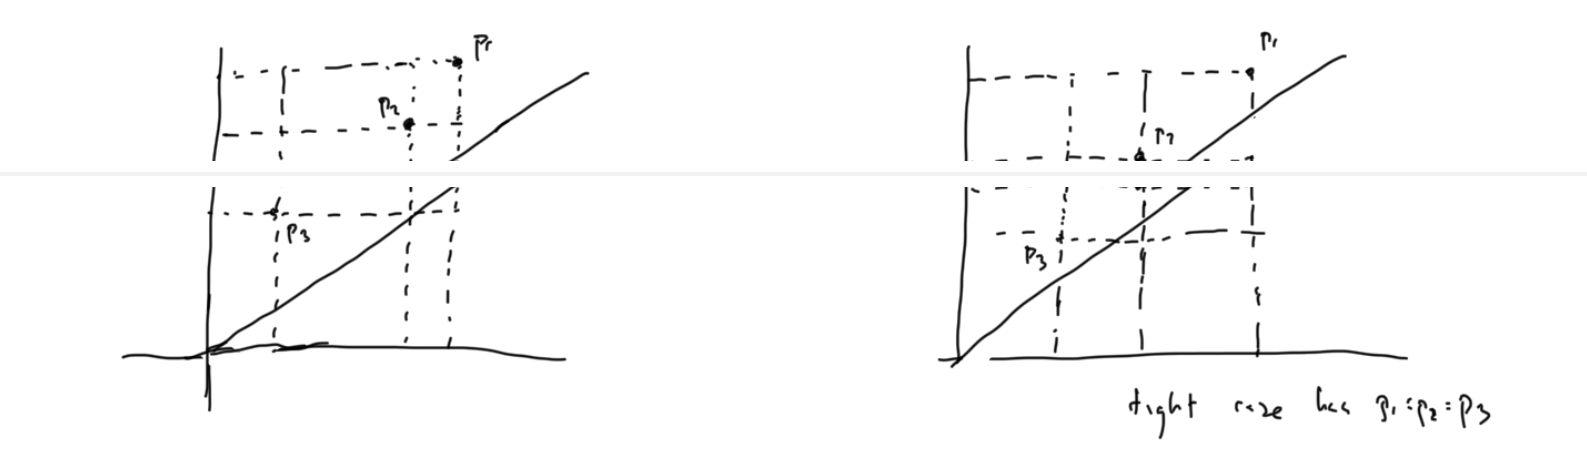
\includegraphics[width=\textwidth]{220103.png}
% \begin{tikzpicture}[scale=1.5]
%   \def\xmin{-1}
%   \def\xmax{3}
%   \def\ymin{\xmin}
%   \def\ymax{\xmax}
%   \draw[->] (\xmin,0) -- (\xmax,0) coordinate (x axis);
%   \draw[->] (0,\ymin) -- (0,\ymax) coordinate (y axis);
%   \draw (\xmin+.5,\ymin+.5) -- (\xmax,\ymax);
%   \node (origin) at (0,0) {};
%   \node (A) at (\xmax-1,\ymax-.3 ) {\textbullet $p_1$};
%   \node (B) at ($ (A) - (.8,.4)$) {\textbullet $p_2$};
%   \node (C) at ($ (A) - (1.3,1.5)$) {\textbullet $p_3$};
%  \foreach \startpoint [count=\i] in {(origin),(A),(B),(C)}{
%    \foreach \endpoint [count=\j] in {(origin),(A),(B),(C)} {
%      \ifnum \i < 5
%      \ifnum \j < 5
%      \draw[dotted] \startpoint -| \endpoint ;
%      % \draw[dashed] \endpoint -- \endpoint |- \startpoint;
%      % \draw[dashed] \startpoint -| \endpoint -- \endpoint;
%      \fi
%      \fi
%       }
%     }
%   \end{tikzpicture}
%   \caption{The case $M=N=1$ and finitely supported $(X,Y)$. The
%     distance between the atoms $p_1$ and $p_2$ is small relative to
%     their distances to the line $x=y$, so they contribute
%     $(p_1+p_2)^2$ to the mass of $\{x<y\}$ under product of the
%     marginals. The distance between $p_1$ and $p_3$ is relatively
%     large, so they contribute only
%     $(p_1+p_3)^2-p_1p_3$.}  \label{fig:inequality}
% \end{figure}


% Theorem \ref{theorem:bounds} extends the inequality to an arbitrary $\P$ so long as $M$ and $N$ are constant.

\begin{theorem}\label{theorem:bounds}
  Let $(X,Y,M,N)\sim \P$ be given as in \eqref{model:cluster auc}. Assume
  further that $M=m$ and $N=n$ are constant. Then
  \begin{align}
    \frac{1}{2}\left(\aucindiv+\frac{\sum_{k,l}\P(X_{1k}=Y_{1l})}{2mn}\right)^2 \le \aucpop \le 1-\frac{1}{2}\left(1-\aucindiv+\frac{\sum_{k,l}\P(X_{1k}=Y_{1l})}{2mn}\right)^2
  \end{align}
  % [[drop 1 and 2 from X/Y observations in favor of primes throughout?]]
\end{theorem}
% Lemma for ($m=n=1$ case).
\noindent The theorem follows from the lemma,
\begin{lemma}\label{lemma:bounds}  Given a pair of scalar random variables $(X,Y)$ with joint distribution $\P$, let $\P_{\cind}$ be the product measure of the marginals, i.e., for all real $a,b$,
  $$
  \P_{\cind}(\{x<a\}\cap\{y<b\})=\P(\{x<a\})\P(\{y<b\}).
  $$
  Then
  \begin{align}
    \frac{1}{2}(\P(X<Y)+\P(X=Y))^2 \le \P_{\cind}(X<Y)+\frac{1}{2}(X=Y)
    \le 1-\frac{1}{2}(1-\P(X<Y))^2.
  \end{align}
\end{lemma}

With the random vector $(X,Y,M,N) \sim \P$, with constant $M=N=1$ so that $\P$ may be regarded as the joint distribution of $(X,Y)$, assumed continuous, the conclusion of the Lemma is
\begin{align}
% $
  \frac{1}{2}(\aucindiv(\P))^2 \le \aucpop(P)
  \le 1-\frac{1}{2}(1-\aucindiv(\P))^2,\label{eqn:lemma:bounds:conclusion}
  % $
\end{align}
equivalently,
\[
1-\sqrt{2(1-\aucpop)} \le \aucindiv \le \sqrt{2\aucpop}.
  \]
When the personalized AUC is completely uninformative, $\aucindiv=1/2$,
the informativity of the population AUC is limited,
$1/8 \le \aucpop \le 7/8$. However, when the population AUC is
completely uninformative, $\aucpop=1/2$, the above bounds on the personalized AUC, which are tight, are vacuous, $0\le\aucindiv\le 1$. Situations as described in Section \ref{section:examples}, where the population AUC $\to 1$ while the personalized AUC $\to 1/2$, appear to require some dependence between $M,N$ and $X,Y$. % Though we do not completely prove this below, giving the bounds not for any $(M,N)\cind (X,Y)$ but specifically for constant $M,N$.








\section{Asymptotic Distribution of $(\aucpop,\aucindiv)$}\label{section:asymptotics}

% stated in greater generality than auc setting. as discussed [[ref]]
% $(\psi,m,n)$ is a sufficient statistic. let $W=(Z,M,N)\sim
% P$. $\Kernel$ is a real-valued function on pairs $(W,W')$ [[domain of
% psi since vectors are variable length??]]  define $\aucpop$ and
% $\aucindiv$ in terms of suff stat ... as well as estimators ... .
Theorem \ref{theorem:asymptotic} gives the asymptotic joint
distribution of the individual and population AUCs. It is stated in
somewhat greater generality for any square-integrable kernel, not just
the AUC kernel \eqref{defn:auc kernel}. The proof is the same for any
random variables $M,N$, such that $\E M\neq 0, \E N\neq 0$,
$\E M^{-2}<\infty,\E N^{-2}<\infty$, i.e., $M$ and $N$ need not be the
lengths of $X$ and $Y$.  Let $\W{i}=(X_i,Y_i,M_i,N_i),i=1,\ldots,\I,$ and let $\seqspace$ denote the space of finite sequences.
\begin{theorem}\label{theorem:asymptotic} Let $\psi:V\times V\to\mathbb{R}$, $(X,Y,M,N)\sim\P$ with $(X,Y)\in V\times V$, $\psi\in L^2(\P)$, $M$ and $N$ counting numbers $> 0$ with finite means. Then:
  \begin{align}
    \sqrt{\I}(\aucpophat-\aucpop,\aucindivhat-\aucindiv) \leadsto \mathcal{N}(0,\Sigma)
  \end{align}
  with
  \begin{align}
    \Sigma_{11} &= \lim_{\I\to\infty} \I\V(\aucpophat) =
    \E\left(\frac{\E(\Kernel_{12}\mid\W{1})+\E(\Kernel_{21}\mid\W{1})}{\E (M)\E (N)} - \aucpop\left(\frac{M_1}{\E (M)} + \frac{N_1}{\E (N)}\right)   \right)^2
    \\
    \Sigma_{22} &= \lim_{\I\to\infty} \I\V(\aucindivhat) =
    \V(\Kernel_{11}/(M_1N_1))
    \\
    \Sigma_{12} &= \lim_{\I\to\infty} \I\cov(\aucpophat,\aucindivhat) =
    \aucpop\E\left(\frac{\Kernel_{11}}{M_1N_1}\left(\frac{\Kernel_{12}+\Kernel_{21}}{\E\Kernel_{12}} - \frac{M_1}{\E (M)}-\frac{N_1}{\E (N)}  \right) \right)
  \end{align}
  % $\sqrt{\I}(\aucpophat-\aucpop,\aucindivhat-\aucindiv) $ converges to a mean-zero bivariate normal distribution with covariance matrix given by
  % \begin{align}
  % \end{align}
\end{theorem}






\begin{corollary}\label{corollary:variance estimator}
  Under the assumptions of Theorem \ref{theorem:asymptotic}, let
  $(X_1,Y_1,M_1,N_1),\ldots,(X_\I,Y_\I,M_\I,N_\I),$ be IID according
  to $\P$. For $1\le i\le \I$ define
  \begin{align}
    \kernel_{i\cdot}&=I^{-1}\sum_{j=1}^\I \kernel(X_i,Y_j),\\
    \kernel_{\cdot i}&=I^{-1}\sum_{j=1}^\I \kernel(X_j,Y_i),\\
    \phi_i &= \frac{\kernel(X_i,Y_i)}{M_iN_i},
  \end{align}
  and analogously for $M_\cdot,N_\cdot,$ and $\kernel_{\cdot\cdot}$. The asymptotic covariance matrix
  $\Sigma$ of $(\aucpophat,\aucindivhat)$ may be consistently
  estimated by $\hat{\Sigma}$ given by:
  \begin{align}
    \hat{\Sigma}_{11} &=\frac{1}{\I-1}\sum_{i=1}^\I\left( \frac{\Kernel_{i\cdot}+\Kernel_{\cdot i}}{M_\cdot N_\cdot}-\aucpophat\left(\frac{M_i}{M_\cdot}+\frac{N_i}{N_\cdot}\right) \right)^2\\
    \hat{\Sigma}_{22} &= \frac{1}{\I-1}\sum_{i=1}^\I(\d_i-\d_\cdot)^2\\
    \hat{\Sigma}_{12} &=\frac{1}{\I}\sum_{i=1}^\I\left(\frac{\d_{i}}{\d_{\cdot}}\left(\frac{\Kernel_{i\cdot}+\Kernel_{\cdot i}}{\Kernel_{\cdot\cdot}} - \frac{M_i}{M_\cdot}-\frac{N_i}{N_\cdot}   \right) \right) %\to_p
  \end{align}
\end{corollary}
\begin{proof}
  See \citet{sen1960} for convergence results for random variables $\Kernel_{i\cdot}$ and $\Kernel_{\cdot i}.$
\end{proof}
The estimator $\hat{\Sigma}_{11}$ of the asymptotic variance of $\aucpophat$ is the same as given by \citet{obuchowski1997}, derived by a different method. The finite-sample performance of this estimator is examined in Section \ref{section:simulation}.



\section{Simulation}\label{section:simulation}

We examine estimation and inference on the population and personalized
AUCs jointly. Many of the choices and parameters follow the simulation
in \citet{obuchowski1997} examining what is here referred to as the
population AUC. Key differences include: 1) In our model
$M>0,N>0,$ to ensure that the personalized AUC is well-defined; 2) Whereas
\citet{obuchowski1997} take $\I=100$, we take the number of clusters to be $\I=\input{sim_coverage_I.txt}$ in the coverage simulation, Section \ref{section:simulation:coverage}, and $\I=10$ in the power simulation, Section \ref{section:simulation:power}.


% \comment{maybe mention many settings similar to obuchowski sim. partially replicates it. key differences: larger cluster sizes. enfoce $M,N>1$. not itnerested in comparison with independence assumption. actually all this is mostly releavnt for the coverage sim not necessarily power sim}

\subsection{Data models}

To generate $(M,N)$, first a preliminary number
$\overline M+\overline N$ of combined case and control observations
belonging in a sample is randomly selected from among
$k\in\{\input{sim_coverage_ks.txt}\}$. Next, to obtain the allocation
to case and control observations, $\overline M+\overline N$ normal
variables are sampled with unit variance and common pairwise
correlation $\rho_{MN}\in\{\input{sim_coverage_corrs.txt}\}$. A
preliminary number $\overline M$ of control observations is taken to
be those greater than $0$, and the remainder the preliminary number
$\overline N$ of case observations. Finally, 1 is added to each to
obtain the final number of control and case observations,
$M=\overline M+1,N=\overline N+1$. The greater the correlation $\rho_{MN}$, the
greater the imbalance between case and control observations within the
clusters.

Two related models were considered for $(X,Y)\mid (M,N)$.

\subsubsection{Bivariate normal model}
A popular parametric model for the AUC is the bivariate normal model, where
the case and control observations are both assumed to follow a normal
distribution \citep{hanley1988}. Following \citet{obuchowski1997} we
extend this model to accommodate clustered data by modeling the
observations as multivariate normal vectors with an exchangeable
correlation structure.
\begin{align}
  (X,Y) \mid (M,N) \sim \mathcal{N}_{M+N}\left(
  % \begin{pmatrix}\mu_X\mathbbm{1}_M\\ \mu_Y\mathbbm{1}_N\end{pmatrix},
    \begin{pmatrix}0\cdot\mathbbm{1}_M\\ \Delta\cdot\mathbbm{1}_N\end{pmatrix},
  \rho\mathbbm{1}_{M+N}\mathbbm{1}_{M+N}^T + (1-\rho)Id_{M+N}
  \right)\label{model:binormal}
\end{align}
That is, the case and control observations of a given cluster all have
unit variance and share the same pairwise correlation $\rho$, all the case observations have mean $\Delta>0$,
and all the control observations mean $0$. The bivariate normal model is in fact an
example of the random effect model described in Section
\ref{section:examples}, though the random effect is not given explicitly in \eqref{model:binormal}. As the impact of the random effect discussed there is only to
change the intra-cluster correlation or mean in \eqref{model:binormal}, it is redundant
to the usual multivariate normal parameters. % Moreover, correlations among control observations or among
% case observations within the same cluster do not contribute to the population or
Moreover, further parameters such as for % intra-cluster control and case correlations
% $\corr(X_{11},X_{12})$, $\corr(Y_{11},Y_{12})$ \comment{really redundant for inference?}, or
for a non-zero control mean $\E(X_{11})$ or non-unit
variances $\V(X_{11})$ and $\V(Y_{11})$ are
redundant for our purpose of modeling AUCs.%\comment{switch to delta parameterization. mux and muy redundant}

% Let $\Delta=\mu_Y-\mu_X\ge 0$.
Using Proposition \ref{proposition:reduction},
\begin{gather}
  \begin{aligned}
  \aucpop(P) &= \Phi\left(\frac{\Delta}{\sqrt{2}}\right)\\
  \aucindiv(P) &=  \Phi\left(\frac{\Delta}{\sqrt{2(1-\rho)}}\right)\label{eqn:binormal formulas}
  % \aucpop(P) &= \Phi\left(\frac{\Delta}{2}\right)\\
  % \aucindiv(P) &=  \Phi\left(\frac{\Delta}{2\sqrt{1-\rho}}\right)\label{eqn:binormal formulas}
\end{aligned}
\end{gather}
The formulas \eqref{eqn:binormal formulas} show that $\aucindiv>\aucpop$ and further that $\aucpop$ and
$\aucindiv$ are simultaneously $>1/2,=1/2,$ or $<1/2$. We give two benefits. The
first is that $(\aucpop,\aucindiv)$ can be restricted without loss of
generality to $[1/2,1]\times[1/2,1]$, switching control and case labels if necessary. The pair $(\aucpop,\aucindiv)$  may then serve as a
parameterization of the bivariate normal model \eqref{model:binormal}, solving for $\Delta$ and $\rho$ in \eqref{eqn:binormal formulas}.  The
second involves testing. Though AUCs are often compared by magnitude% \comment{cite multi-reader papers}
, e.g., $H_0:AUC_1-AUC_2>0$, one is
usually interested in the discrimination, i.e., $|AUC_1-1/2|$ versus
$|AUC_2-1/2|$. The hypothesis $H_0:AUC_1-AUC_2>0$ is ambiguous, indicating that
$AUC_1$ than is more discriminating than $AUC_2$ when both are greater than $1/2$, but less
discriminating if both are less than $1/2$.  A further complication, which will not
be solved by switching the class designations, is
that one AUC may be greater than $1/2$ and the other less. These complications are
avoided in the bivariate normal model for the personalized and population
AUCs. A test of $\aucpop=\aucindiv$ versus $\aucpop<\aucindiv$ is also a test of
discrimination, $|\aucpop-1/2|=|\aucindiv-1/2|$ versus $|\aucpop-1/2|<|\aucindiv-1/2|$.

\subsubsection{Censored bivariate normal model}

We also examine the bivariate normal model under censoring, a mixed
discrete-continuous distribution. Let $\bnd>0$, let
$(\overline X,\overline Y)\mid (M,N)$ be sampled as in in
\eqref{model:binormal}, and let
\begin{gather}
  \begin{aligned}
    \label{model:censored binormal}
  &(X,Y) \mid (M,N) =(-\bnd\{\overline{X}\le-\bnd\}+\overline X\{-\bnd<\overline X <\bnd\} + a\{\overline X\ge a\},\\
  &\qquad
  -\bnd\{\overline{Y}\le-\bnd\}+\overline Y\{-\bnd<\overline Y <\bnd\} + a\{\overline Y\ge a\}).
\end{aligned}
\end{gather}
That is, observations $(\overline X,\overline Y)$ are generated as in the bivariate normal model
\eqref{model:binormal}, and the values are then clipped to $\pm \bnd$.
This type of data-generating process is used by \citet{obuchowski1997} to model
radiologists' scores, which lie on a 0---100\% scale and often
accumulate at $0\%$ and $100\%$.

Let
$$(X_{11},Y_{11})\sim \mathcal{N}_2\left(\begin{pmatrix} 0 \\ \Delta \end{pmatrix},
  \begin{pmatrix} 1 & \rho \\ \rho & 1 \end{pmatrix}
\right).$$
Again using Proposition \ref{proposition:reduction} to reduce to the $M=N=1$ case,
\begin{align}
  \aucpop(P) &=-\int_{-\bnd}^\bnd\Phi(x-\Delta)\phi(x)dx + \frac12(\Phi(\bnd)-\Phi(\bnd-\Delta)-\Phi(-\bnd-\Delta)\\
  &\qquad+\Phi(\bnd)(\Phi(-\bnd-\Delta)+\Phi(\bnd-\Delta))+1)\\
  \aucindiv(P) &=\int_{-\bnd}^\bnd\int_x^\bnd f_{X_{11},Y_{11}}(x,y)dydx + \Phi(-a) + 1 - \Phi(\bnd-\Delta) - \frac12 P(X_{11}<-\bnd,Y_{11}<-\bnd)\\
  &\qquad - \frac12 P(X_{11}>\bnd,Y_{11}>\bnd) - P(X_{11}< -\bnd, Y_{11}>\bnd).
\end{align}
Due to the censoring, the AUCs may be bounded below $1$ in this
model, regardless of the magnitude of the location shift between the underlying control and
case observations. As $\Delta\to\infty$, $\aucpop$ and $\aucindiv$
both tend to $\frac12(1+\Phi(\bnd))$.


\subsection{Coverage}\label{section:simulation:coverage}

% Given $M$ and $N$, the control and case observations $X$ and $Y$
% were sampled according to [[ref display]].
The parameters $\Delta$ and
$\rho$ were set to correspond to a population AUC of $\aucpop\in\{\input{sim_coverage_theta.12s.txt}\}$ and
personalized AUCs of $\aucindiv\in\{\input{sim_coverage_theta.11s.txt}\}$ with $\aucindiv\ge\aucpop$. For each setting of $\rho_{MN},\aucpop,\aucindiv$, $\input{sim_coverage_reps.txt}$ replicates
of size $\I=\input{sim_coverage_I.txt}$ were sampled and used to form a confidence ellipse for
$(\aucpop,\aucindiv)$. Specifically, with $\aucpophat,\aucindivhat$ computed as
in Section \ref{section:setting} and $\Sigma$ as in Theorem \ref{theorem:asymptotic}, under $P$,
\begin{align}
\bigg\vert\Sigma^{-1/2}\left(\begin{pmatrix}\aucpop\\
\aucindiv\end{pmatrix}-\begin{pmatrix}\aucpophat\\\aucindivhat\end{pmatrix}\right)\bigg\vert^2\label{eqn:simulation:confidence region}
\end{align}
has a chi-squared distribution with 2 degrees of freedom. If
$q$ is an upper $\alpha$ quantile of this distribution, then
$$
\left\{\begin{pmatrix}x\\y\end{pmatrix}:\bigg\vert\Sigma^{-1/2}\left(\begin{pmatrix}x\\y\end{pmatrix}-\begin{pmatrix}\aucpophat\\\aucindivhat\end{pmatrix}\right)\bigg\vert^2
< q\right\}
$$
is a level $1-\alpha$ confidence region for $(\aucpop,\aucindiv)$, which then
covers $(\aucpop,\aucindiv)$ when \eqref{eqn:simulation:confidence region} is $<q$. In the simulation, we substitute for $\Sigma$ the asymptotic approximation $\hat\Sigma$ given in Corollary \ref{corollary:variance estimator}.
% This process was repeated $[[...]]$ times.
Results are presented in Table
\ref{table:1}. The bias is on the order of a hundredth at this sample size, and the coverage is generally close to .95. There is some degradation in the coverage as $(\aucpop,\aucindiv)$ approach $(1,1)$.


\begin{table}
  \subfloat[Binormal model \eqref{model:binormal}]{
    \begin{tabular}{rrrrrrrrrr}
  \hline
 & theta.12 & theta.11 & D.corr & coverage & bias.theta.11 & bias.theta.12 & vcov.11 & vcov.12 & vcov.22 \\ 
  \hline
1 & 0.60 & 0.60 & 0.00 & 0.90 & 0.01 & 0.00 & -0.04 & -0.03 & -0.02 \\ 
  2 & 0.60 & 0.60 & 0.40 & 0.97 & 0.00 & 0.00 & -0.01 & 0.00 & 0.00 \\ 
  3 & 0.60 & 0.60 & 0.80 & 0.93 & -0.00 & -0.00 & 0.03 & 0.01 & 0.01 \\ 
  4 & 0.60 & 0.60 & 0.95 & 0.90 & -0.01 & 0.00 & -0.05 & -0.02 & -0.01 \\ 
  1.1 & 0.60 & 0.77 & 0.00 & 0.97 & -0.00 & -0.00 & 0.01 & -0.00 & 0.00 \\ 
  2.1 & 0.60 & 0.77 & 0.40 & 1.00 & 0.00 & 0.00 & 0.00 & 0.00 & 0.03 \\ 
  3.1 & 0.60 & 0.77 & 0.80 & 0.97 & 0.00 & -0.00 & 0.01 & -0.00 & 0.05 \\ 
  4.1 & 0.60 & 0.77 & 0.95 & 0.90 & 0.01 & 0.01 & -0.01 & -0.02 & -0.02 \\ 
  1.2 & 0.60 & 0.95 & 0.00 & 1.00 & 0.00 & -0.00 & 0.00 & 0.00 & -0.00 \\ 
  2.2 & 0.60 & 0.95 & 0.40 & 0.87 & 0.00 & 0.00 & -0.00 & -0.00 & -0.03 \\ 
  3.2 & 0.60 & 0.95 & 0.80 & 1.00 & 0.00 & 0.00 & 0.00 & 0.00 & -0.01 \\ 
  4.2 & 0.60 & 0.95 & 0.95 & 0.97 & -0.00 & 0.01 & 0.00 & -0.01 & -0.01 \\ 
  1.3 & 0.80 & 0.80 & 0.00 & 0.90 & 0.00 & 0.00 & 0.00 & 0.00 & -0.00 \\ 
  2.3 & 0.80 & 0.80 & 0.40 & 0.93 & -0.00 & 0.00 & 0.01 & -0.00 & -0.00 \\ 
  3.3 & 0.80 & 0.80 & 0.80 & 0.90 & 0.00 & 0.00 & -0.01 & -0.00 & 0.00 \\ 
  4.3 & 0.80 & 0.80 & 0.95 & 0.93 & -0.00 & 0.00 & -0.02 & 0.00 & 0.00 \\ 
  1.4 & 0.80 & 0.88 & 0.00 & 0.97 & -0.00 & 0.00 & 0.00 & 0.00 & 0.01 \\ 
  2.4 & 0.80 & 0.88 & 0.40 & 0.93 & -0.00 & 0.01 & 0.00 & 0.00 & 0.00 \\ 
  3.4 & 0.80 & 0.88 & 0.80 & 0.87 & 0.01 & 0.01 & 0.01 & 0.01 & -0.01 \\ 
  4.4 & 0.80 & 0.88 & 0.95 & 0.90 & 0.01 & 0.01 & 0.01 & 0.01 & 0.00 \\ 
  1.5 & 0.80 & 0.95 & 0.00 & 0.93 & 0.00 & 0.00 & 0.00 & 0.00 & 0.01 \\ 
  2.5 & 0.80 & 0.95 & 0.40 & 1.00 & -0.00 & -0.00 & 0.00 & -0.00 & 0.02 \\ 
  3.5 & 0.80 & 0.95 & 0.80 & 0.90 & -0.00 & -0.00 & 0.00 & 0.01 & 0.00 \\ 
  4.5 & 0.80 & 0.95 & 0.95 & 1.00 & -0.00 & -0.00 & 0.00 & -0.00 & 0.01 \\ 
   \hline
\end{tabular}
 
 % \caption{}
  % \label{table:1}
    }
  \\
    \subfloat[Binormal model with censoring \eqref{model:censored binormal}]{\begin{tabular}{|C{1.4cm}|C{1.4cm}|C{1.4cm}||C{1.4cm}||C{1.4cm}|C{1.4cm}|C{1.4cm}|C{1.4cm}|C{1.4cm}|}
  \hline
  \multicolumn{3}{|c||}{parameters} & coverage &\multicolumn{5}{c|}{bias} \\
 \hline
 \hline
 $\theta_{12}$ & $\theta_{11}$ & $\rho_{MN}$ &  & $\theta_{12}$ & $\theta_{11}$  & $\Sigma_{11}$ & $\Sigma_{12}$ & $\Sigma_{22}$ \\
 \hline
0.70 & 0.70 & 0.00 & 0.94 & 0.00 & 0.00 & 0.00 & 0.00 & 0.00 \\ 
  0.70 & 0.70 & 0.10 & 0.94 & 0.00 & 0.00 & -0.00 & 0.00 & 0.01 \\ 
  0.70 & 0.70 & 0.40 & 0.93 & 0.00 & 0.00 & -0.00 & -0.01 & -0.00 \\ 
  0.70 & 0.70 & 0.80 & 0.94 & 0.00 & 0.00 & -0.00 & -0.00 & -0.00 \\ 
  0.70 & 0.80 & 0.00 & 0.94 & 0.00 & 0.00 & 0.00 & -0.00 & -0.00 \\ 
  0.70 & 0.80 & 0.10 & 0.91 & 0.00 & 0.00 & -0.01 & -0.00 & -0.01 \\ 
  0.70 & 0.80 & 0.40 & 0.94 & 0.00 & -0.00 & 0.00 & 0.00 & 0.00 \\ 
  0.70 & 0.80 & 0.80 & 0.93 & 0.00 & 0.00 & 0.00 & -0.00 & -0.00 \\ 
  0.80 & 0.80 & 0.00 & 0.94 & 0.00 & -0.00 & 0.00 & 0.00 & 0.00 \\ 
  0.80 & 0.80 & 0.10 & 0.93 & 0.00 & -0.00 & 0.00 & 0.00 & 0.00 \\ 
  0.80 & 0.80 & 0.40 & 0.95 & -0.00 & -0.00 & 0.00 & -0.00 & 0.00 \\ 
  0.80 & 0.80 & 0.80 & 0.92 & 0.00 & -0.00 & -0.01 & -0.00 & -0.00 \\ 
  0.80 & 0.90 & 0.00 & 0.93 & 0.00 & -0.01 & -0.00 & -0.00 & 0.00 \\ 
  0.80 & 0.90 & 0.10 & 0.92 & 0.00 & -0.01 & -0.00 & -0.00 & -0.00 \\ 
  0.80 & 0.90 & 0.40 & 0.92 & 0.00 & -0.01 & -0.00 & -0.00 & 0.00 \\ 
  0.80 & 0.90 & 0.80 & 0.93 & 0.00 & -0.01 & 0.00 & 0.00 & 0.01 \\ 
   \hline
\end{tabular}
}
      %       \label{table:2}
    \caption{The results of a simulation examining the coverage of a nominal 95\% confidence ellipse obtained using the asymptotic estimator given in Section \ref{section:asymptotics}.\comment{make conssitent order of theta11 vs theta12 columns} For $\aucindiv$ and $\aucpop$, the bias is computed as the mean difference between the estimates and the known true values. For the elements of the covariance matrix $\Sigma_{ij}$, the bias is the mean difference between the estimates given by Theorem \ref{theorem:asymptotic}   and the empirical covariance.}
    \label{table:1}
\end{table}

% \begin{table}
%   \begin{tabular}{|C{1.4cm}|C{1.4cm}|C{1.4cm}||C{1.4cm}||C{1.4cm}|C{1.4cm}|C{1.4cm}|C{1.4cm}|C{1.4cm}|}
  \hline
  \multicolumn{3}{|c||}{parameters} & coverage &\multicolumn{5}{c|}{bias} \\
 \hline
 \hline
 $\theta_{12}$ & $\theta_{11}$ & $\rho_{MN}$ &  & $\theta_{12}$ & $\theta_{11}$  & $\Sigma_{11}$ & $\Sigma_{12}$ & $\Sigma_{22}$ \\
 \hline
0.70 & 0.70 & 0.00 & 0.94 & 0.00 & 0.00 & 0.00 & 0.00 & 0.00 \\ 
  0.70 & 0.70 & 0.10 & 0.94 & 0.00 & 0.00 & -0.00 & 0.00 & 0.01 \\ 
  0.70 & 0.70 & 0.40 & 0.93 & 0.00 & 0.00 & -0.00 & -0.01 & -0.00 \\ 
  0.70 & 0.70 & 0.80 & 0.94 & 0.00 & 0.00 & -0.00 & -0.00 & -0.00 \\ 
  0.70 & 0.80 & 0.00 & 0.94 & 0.00 & 0.00 & 0.00 & -0.00 & -0.00 \\ 
  0.70 & 0.80 & 0.10 & 0.91 & 0.00 & 0.00 & -0.01 & -0.00 & -0.01 \\ 
  0.70 & 0.80 & 0.40 & 0.94 & 0.00 & -0.00 & 0.00 & 0.00 & 0.00 \\ 
  0.70 & 0.80 & 0.80 & 0.93 & 0.00 & 0.00 & 0.00 & -0.00 & -0.00 \\ 
  0.80 & 0.80 & 0.00 & 0.94 & 0.00 & -0.00 & 0.00 & 0.00 & 0.00 \\ 
  0.80 & 0.80 & 0.10 & 0.93 & 0.00 & -0.00 & 0.00 & 0.00 & 0.00 \\ 
  0.80 & 0.80 & 0.40 & 0.95 & -0.00 & -0.00 & 0.00 & -0.00 & 0.00 \\ 
  0.80 & 0.80 & 0.80 & 0.92 & 0.00 & -0.00 & -0.01 & -0.00 & -0.00 \\ 
  0.80 & 0.90 & 0.00 & 0.93 & 0.00 & -0.01 & -0.00 & -0.00 & 0.00 \\ 
  0.80 & 0.90 & 0.10 & 0.92 & 0.00 & -0.01 & -0.00 & -0.00 & -0.00 \\ 
  0.80 & 0.90 & 0.40 & 0.92 & 0.00 & -0.01 & -0.00 & -0.00 & 0.00 \\ 
  0.80 & 0.90 & 0.80 & 0.93 & 0.00 & -0.01 & 0.00 & 0.00 & 0.01 \\ 
   \hline
\end{tabular}

%   \caption{binormal censored model}
%   \label{table:2}
% \end{table}

% \comment{TODO: % 1. similar simulation performed with truncated normal or other nonnormal distr. 2.
%   check M,N imbalance affects precision as in obuchowski.}


\subsection{Power}\label{section:simulation:power}

We examine the power of testing the null hypothesis
$H_0:\aucpop=\aucindiv$ using the proposed variance estimators under
the bivariate normal model \eqref{model:binormal}. Restricting to $\rho>0$ in
\eqref{model:binormal}, the set of alternatives to $H_0:1/2< \aucpop=\aucindiv$ is
 $H_A:1/2<\aucpop<\aucindiv$, i.e., where the
personalized AUC is more discriminating than the population AUC.

The data is generated under \eqref{model:binormal} using
$(\aucpop,\aucindiv)$ selected from points randomly and uniformly selected in
$[\frac{1}{2},1]\times[\frac{1}{2},1], \{\aucindiv\ge\aucpop\}$. Estimates
$\aucpophat,\aucindivhat,$ and $\hat\Sigma$ were then obtained as described
above. The test is carried out by testing the significance of the
z-statistic
$$
% (\aucpophat-\aucindivhat) /
% \sqrt{\begin{pmatrix}1&-1\end{pmatrix}^T\hat\Sigma\begin{pmatrix}1\\-1\end{pmatrix}}
(\aucpophat-\aucindivhat) /
\sqrt{c^t\hat\Sigma c}
$$
where the contrast vector $c$ is $(1,-1)^t$.



The observed power functions are plotted in Fig. \ref{fig:power}. The
number of clusters was chosen to be $\I=10$, few relative to the setting in
\citet{obuchowski1997} % or the number encountered in the data in Section
% \ref{section:data analysis}
, since the qualitative behavior of the power surface appears
clearer with fewer clusters. \comment{give some summary of results
  maybe.}


% \begin{table}
%   \subfloat[Binormal model \eqref{model:binormal}]{
%   \includegraphics[width=5cm]{../sim/220813/a/220813.pdf}
%  % \caption{}
%   % \label{table:1}
%     }

%     \subfloat[Binormal model with censoring \eqref{model:censored binormal}]{
%     \includegraphics[width=5cm]{../sim/220813/b/220813.pdf}
%   }
%       %       \label{table:2}
%     \caption{The results of a simulation examining the coverage of a nominal 95\% confidence ellipse obtained using the asymptotic estimator given in Section \ref{section:asymptotics}.\comment{make conssitent order of theta11 vs theta12 columns}. For $\aucindiv$ and $\aucpop$, the bias is computed as the mean difference between the estimates and the known true values. For the elements of the covariance matrix $\Sigma_{ij}$, the bias is the mean difference between the estimates given by Theorem \ref{theorem:asymptotic}   and the empirical covariance.}
%     \label{table:1}
% \end{table}


% \begin{figure}
%   \centering
%   \begin{tabular}[b]{c}
%     \includegraphics[width=.4\linewidth]{../sim/220813/a/220813.pdf} \\
%     \small (a)
%   \end{tabular} \qquad
%   \begin{tabular}[b]{c}
%     \includegraphics[width=.4\linewidth]{../sim/220813/b/220813.pdf} \\
%     \small (b)
%   \end{tabular}
%   \caption{Comparison of steady state results (a)~x method (b)~y method}
% \end{figure}

\begin{figure}[!tbp]
  \centering
  % \subfloat[Bivariate normal model \eqref{model:binormal}]{\includegraphics[width=0.5\textwidth]{../sim/220813/a/220813.pdf}}
  \subfloat[Bivariate normal model \eqref{model:binormal}]{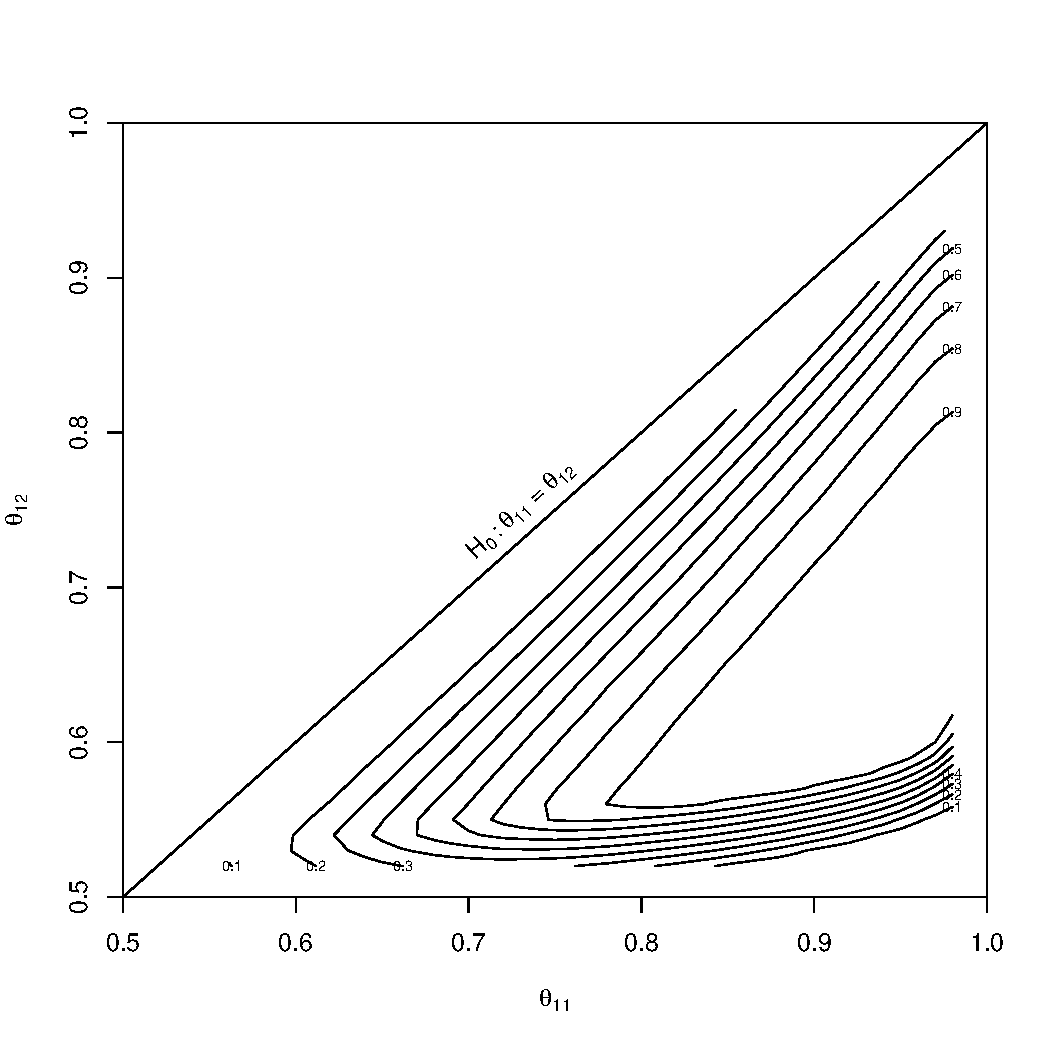
\includegraphics[width=0.5\textwidth]{220813a.pdf}}
  \hfill
  % \subfloat[Bivariate normal model with censoring \eqref{model:censored binormal}]{\includegraphics[width=0.5\textwidth]{../sim/220813/b/220813.pdf}}
  \subfloat[Bivariate normal model with censoring \eqref{model:censored binormal}]{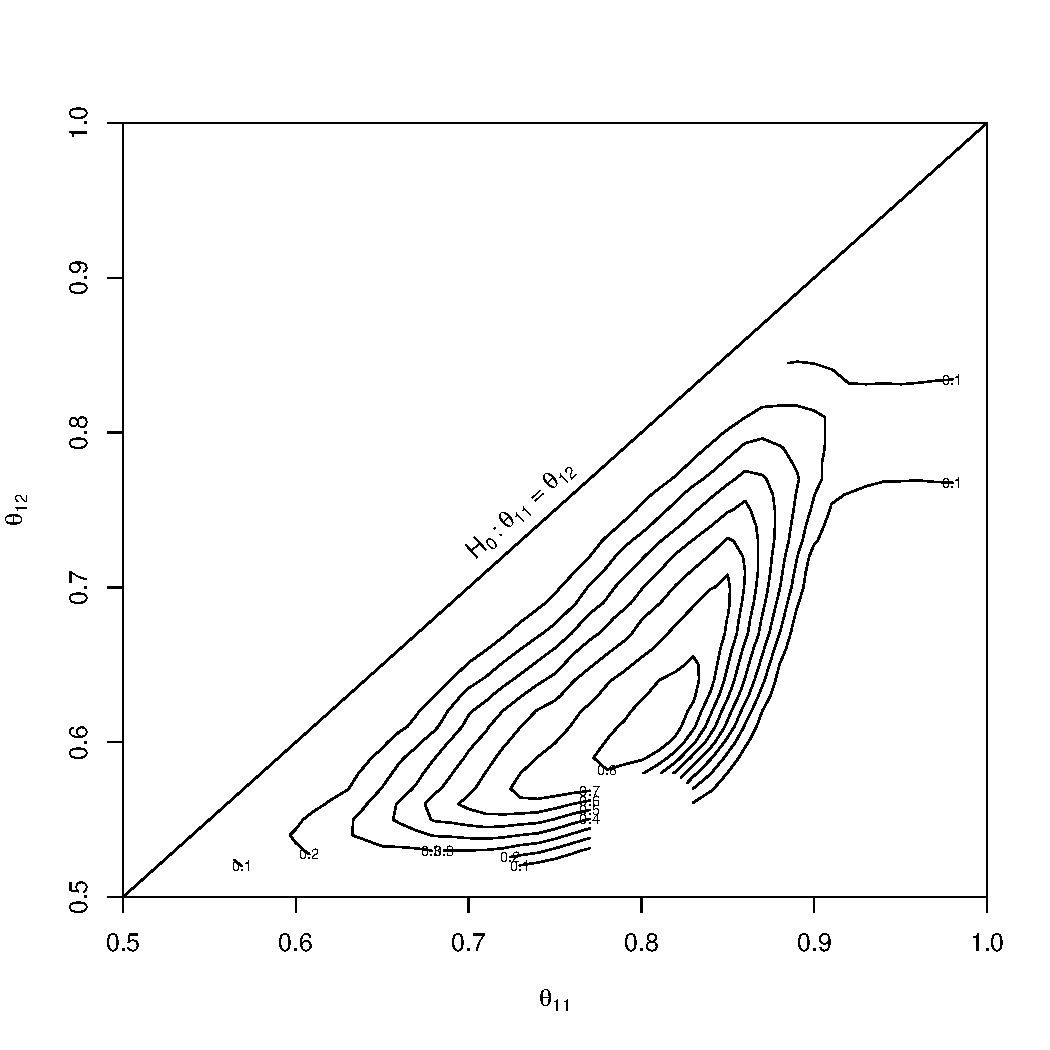
\includegraphics[width=0.5\textwidth]{220813b.pdf}}
  \caption{Empirical power function of the test of $H_0:\aucpop=\aucindiv$ versus $\aucpop<\aucindiv$ using the
     asymptotic estimator given in Section
     \ref{section:asymptotics}. In the bivariate normal model with or without censoring, the null is equivalent to $H_0:|\aucpop-1/2|=|\aucindiv-1/2|,$ equal informativity.}  \label{fig:power}
\end{figure}

% \begin{figure}
%   \centering
%   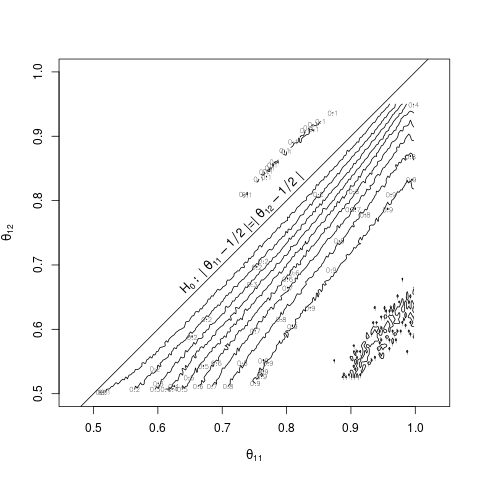
\includegraphics{../sim/211120/211120.png}
%   \caption{Power of the test of $H_0:\aucpop=\aucindiv$ using the
%     asymptotic estimator given in Section
%     \ref{section:asymptotics}. \comment{put null in usual format,get rid of
%     artifacts, more monte carlo interations to smooth out}} \label{fig:power}
% \end{figure}



% difference in magnitude of ind and pop versus difference in
% informativity. same for this example.

% give power surfaces.

% should have table besides figure.
% should have something with (m,n) confounding. maybe geenral setting?



\section{Discussion}\label{section:conclusion}
We have compared and contrasted two generalizations of the AUC to
accommodate clustered, paired data. Straightforward extensions include allowing
for multiple dependent AUCs, clusters that are only exchangeable or
otherwise fall short of being IID, and covariate-adjusted AUCs. A more
delicate extension would allow for estimation of the personalized AUC
when some clusters have no control or no case observations.  As the
personalized AUC is not currently defined for such clusters either the
definition would need to be re-worked or a model would need to be
introduced for the missing values corresponding to those clusters. No
major changes would be required of the analysis under a
strong enough assumption such as ignorability, i.e., the assumption that the behavior of the
personalized AUC (or the pair) is the same on $M>1,N>1$ as on the
entire population. \comment{cite to data analysis for pop auc as an
  example, if that analysis gets completed}

% Directions for future work:
% \begin{enumerate}
% \item multiple correlated AUCs--easy extension of the above results\comment{application: lehman berkeley data?}. e.g. testing simultaneously whether two biomarkers/predictors differ as to either the population or personalized aucs.
% \item allow for clusters without either case or control
%   observations. will need a model for missingness. with a strong
%   enough assumption like ignorability can just use the $M>1,N>1$
%   definition given here with minor modifications. personalized auc
%   stilll woudlnt be estimable with data wehre units were all case or
%   all control.
% \item longitudinal analysis
% \item covariate-adjusted AUC
%   \item non-IID clusters
% \end{enumerate}



\bibliographystyle{apalike}
\bibliography{auc.bib}







  \begin{proof}[Proof of Proposition \ref{proposition:aucpop}]
    \begin{enumerate}
    \item By the LLN $\I^2/MN \to 1/(\E (M)\E (N))$ almost surely and by Lemma \ref{corollary:convergence} $\sum_{i,j}\Kernel_{ij}/\I^2 \to \E \Kernel_{12}$ almost surely. Conditioning on the sample,
      \begin{align}
        \E \kernel(\xi_\I,\eta_\I) &= \E( \E (\kernel(\xi_\I,\eta_\I) \mid (X_1,Y_1,M_1,N_1),\ldots,(X_\I,Y_\I,M_\I,N_\I))\\
                                   &= \E\left(\frac
                                     {\sum_{1\le i,j\le\I}\sum_{1\le k\le M_i,1\le l\le N_j}\kernel(X_{ik},Y_{jl})}
                                     {\sum_{i=1}^\I M_i \sum_{i=1}^\I N_i} \right)\\
                                   &= \E\left(\frac{\sum_{1\le i,j\le\I}\Kernel_{ij}}{\sum_{i=1}^\I M_i \sum_{i=1}^\I N_i} \right) \to \frac{\E\Kernel_{12}}{\E (M) \E (N)}=\aucpop.
      \end{align}
      The limit is justified since $\sum_{i,j}\psi_{i,j}/(\sum_i M_i\sum_i N_i)\le 1$. %dominated convergence, given the boundedness of $\I^2/MN$ and moment condition on $\Kernel$.

    \item The second part follows on showing that $(\xi_\I,\eta_\I)\to (\xi_\infty,\eta_\infty)$ setwise. % \comment{if arguing $\theta_{12}(P_\I)\to\theta_{12}(P_\infty)$ need to show $P_\I$ concentrates on a continuity set of $P_\infty$.}
      For $a,b\in\mathbb{R}$, by a similar argument as above,
      \begin{align}
        \P(\xi_\I<a,\eta_\I<b) &=\E\left(\frac
                                     {\sum_{1\le i,j\le\I}\sum_{1\le k\le M_i,1\le l\le N_j}\{X_{ik}<a,Y_{jl}<b\}}
                                 {\sum_{i=1}^\I M_i \sum_{i=1}^\I N_i} \right)\\
                               &\to \frac{\E\left(\sum_{k=1}^{M_1}\{X_{1k}<a\}\right)}{\E (M)}
                                 \frac{\E\left(\sum_{l=1}^{N_1}\{Y_{1l}<b\}\right)}{\E (N)}.
      \end{align}
      The probability of sampling an element from a cluster of size
      $M=m$ given an initial segment of $\I$ samples
      $(X_1,Y_1,M_1,N_1),\ldots,(X_\I,Y_\I,M_\I,N_\I),$ is
      $\frac{m\sum_{i=1}^\I\{M_i=m\}}{\sum_{i=1}^\I M_i}$. Along almost
      any sequence of samples as $\I\to\infty$ this relative frequency
      tends to $\frac{m\P(M=m)}{\E (M)}$. Therefore
      \begin{align}
        \P(\xi_\infty < a) &= \sum_{m=1}^\infty\P(\xi_\infty < a \mid \xi_\infty\text{ is sampled from a cluster of size }m)\cdot\\
        &\hspace{.5in}\P(\xi_\infty\text{ is sampled from a cluster of size }m)\\
                           &= \sum_{m=1}^\infty\frac{1}{m}\sum_{k=1}^m\P(X_{1k}<a\mid M=m)\frac{m\P(M=m)}{\E (M)}\\
                           &=\frac{1}{\E M}\sum_{m=1}^\infty\sum_{k=1}^m\P(X_{1k}<a\mid M=m)\P(M=m)\\
        &=\frac{1}{\E (M)}\E\left(\sum_{k=1}^M\{X_{1k}<a\}\right).
      \end{align}
      Analogously,
      $$
      \P(\eta_\infty < a)=\frac{1}{\E (N)}\E\left(\sum_{l=1}^N\{X_{1l}<a\}\right).
      $$
      The product is the limit of
      $\P(\xi_\I<a,\eta_\I<b)$ given above.
    \end{enumerate}
  \end{proof}
    The following lemma gives a convergence result for a two-sample $U$-statistic with kernel of degree $(1,1)$ where the data is paired. The corresponding definitions and result for independent samples is given in, e.g., \citet{lee2019}. Let $\seqspace$ denote the space of finite sequences.%\comment{Need to define $V$, the space where $X,Y$ lie. These are vectors of variable length so $V$ should be at least as big as $c_{00}$}

  %   \begin{lemma}\label{lemma:hajek} Given a sample $(X_0,Y_0),(X_1,Y_1),\ldots,(X_\I,Y_\I)$ on
  %   $\seqspace\times\seqspace$ IID according to $\P$ and a
  %   function $\Kernel: \seqspace\times\seqspace \to \mathbb{R}$ in $L^2(\P)$, define
  %   $$
  %   U_\I = \I^{-2}\sum_{1\le i,j\le\I}\Kernel(X_i,Y_j)
  %   $$
  %   and
  %   $$
  %   \hat{U}_\I = \I^{-1}\sum_{i=1}^\I\left(\E(\Kernel(X_i,Y_0)\mid X_i,Y_i) + \E(\Kernel(X_0,Y_i)\mid X_i,Y_i)\right) - 2\E\Kernel(X_1,Y_2).
  %   $$
  %   Then
  %   $$
  %   \E(U_\I-\E U_\I-\hat{U}_\I)^2=O(\I^{-2}).
  %   $$
  % \end{lemma}

  % \begin{proof}[Proof of Lemma \ref{lemma:hajek}]

  %   Let $V_\I=(\I)^{-1}_2\sum_{\stackrel{1\le i,j\le \I}{i\neq j}}\psi_{ij}.$ Then,

  %   \begin{align}
  %     \E(V_\I-\E\Kernel_{12})^2 &= (\I_2)^{-2}\E(\sum_{i\neq j}\Kernel_{ij})^2-\left(\E\Kernel_{12}\right)^2\\%...\V\left( (\I)_2^{-1}\sum_{i\neq j}\Kernel_{ij}\right) \\
  %                               &= \frac{\I-2}{\I(\I-1)}\left(\E\Kernel_{12}\Kernel_{13}+\E\Kernel_{12}\Kernel_{13}+2\E\Kernel_{12}\Kernel_{31}\right) + \left(\frac{(\I)_4}{(\I)^2_2}-1\right)\left(\E\Kernel_{12}\right)^2+O(\I^{-2})\\
  %                               &= \frac{\I-2}{\I(\I-1)}\left(\I\E\hat{U}_\I^2+4\left(\E\Kernel_{12}\right)^2 \right) + \left(\frac{(\I)_4}{(\I)^2_2}-1\right)\left(\E\Kernel_{12}\right)^2+O(\I^{-2})\\
  %                                                           % \\&=...\V(\E(\Kernel(X_1,Y_0)\mid X_1,Y_1)+\E(\Kernel(X_0,Y_1)\mid X_1,Y_1))\\
  %                                                           &=\frac{\I-2}{\I-1}\V(\hat{U}_\I) + O(\I^{-2}).
  %   \end{align}
  %   By a similar computation, or by viewing $\hat{U}_\I$ as the H\'ajek projection of $V_\I$ \cite{lee2019},
  %   \begin{align}
  %     \E\left((V_\I-\E\Kernel_{12})\hat{U}_\I\right)=\E\hat{U}_\I^2.
  %   \end{align}
  %   % \begin{align}
  %   %   &\cov(\Kernel_{12},\E(\Kernel(X_1,Y_0)\mid X_1,Y_1)+\E(\Kernel(X_0,Y_1)\mid X_1,Y_1)+\E(\Kernel(X_2,Y_0)\mid X_2,Y_2)+\E(\Kernel(X_0,Y_2)\mid X_2,Y_2))\\
  %   %   &\qquad = ...\\
  %   %   &\qquad = \V(\E(\Kernel(X_1,Y_0)\mid X_1,Y_1)+\E(\Kernel(X_0,Y_1)\mid X_1,Y_1))\\
  %   %   &\qquad=\I\V(\hat{U}_\I).
  %   % \end{align}
  %   The variance of the IID sum $\hat{U}_\I$ is $O(\I^{-1})$. Therefore,
  %   \begin{align}
  %     \E\left(U_\I-\E U-\hat{U}_\I\right)^2 &= \E\left(V_\I-\E\Kernel_{12}-\hat{U}_\I\right)^2 +  O(\I^{-2})\\
  %                                           &= \left(\frac{\I-2}{\I-1}-2+1\right)\E\hat{U}_\I^2 + O(\I^{-2})\\
  %                                           &= O(\I^{-2}).
  %   \end{align}
  % \end{proof}

    \begin{lemma}\label{lemma:hajek} Given a sample $(X_0,Y_0),(X_1,Y_1),\ldots,(X_\I,Y_\I)$ on
    $\seqspace\times\seqspace$ IID according to $\P$ and a
    function $\Kernel: \seqspace\times\seqspace \to \mathbb{R}$ in $L^2(\P)$, define
    $$
    U_\I = \I^{-2}\sum_{\substack{1\le i,j\le\I\\i\neq j}}\Kernel(X_i,Y_j),\qquad
    V_\I = \I^{-2}\sum_{1\le i,j\le\I}\Kernel(X_i,Y_j),
    $$
    and
    $$
    \hat{U}_\I = \I^{-1}\sum_{i=1}^\I\left(\E(\Kernel(X_i,Y_0)\mid X_i,Y_i) + \E(\Kernel(X_0,Y_i)\mid X_i,Y_i)\right) - 2\E\Kernel(X_1,Y_2).
    $$
    Then
    $$
    \E(U_\I-\E U_\I-\hat{U}_\I)^2=O(\I^{-2})\text{ and }  \E(V_\I-\E V_\I-\hat{U}_\I)^2=O(\I^{-2}).
    $$
  \end{lemma}

  \begin{proof}[Proof of Lemma \ref{lemma:hajek}]

    Define
    $$
    \overline\Kernel_{ij}=\Kernel(X_i,Y_j) - \E(\Kernel(X_i,Y_0)\mid X_i,Y_i) - \E(\Kernel(X_0,Y_j)\mid X_j,Y_j) + \E\Kernel(X_0,Y_0).
    $$
    Then, for $i\neq j$, $\E (\overline\Kernel_{ij}\mid (X_i,Y_i))=\E (\overline\Kernel_{ij}\mid (X_j,Y_j))=0$, implying
    \begin{align}
      \E(U_\I-\E U_\I - \hat{U}_\I)^2 &= \E\left((\I)^{-1}_2\sum_{i\neq j} \overline\Kernel_{ij}\right)\\
                                      &= (\I)_2^{-2}\sum_{i\neq j}\E \overline\Kernel_{ij}^2 + O(\I^{-2})\\
                                      &=O(\I^{-2}).
    \end{align}

    For the second equation,
    \begin{align}
      \E(U_\I-\E U_\I - V_\I+\E V_\I)^2 &=  \I^{-2}\E\left((\I)_2^{-1}\sum_{i\neq j}\Kernel_{ij} - \E \Kernel_{11}+\E\Kernel_{12}\right)^2\\
                                        &\le \I^{-2}\left((\I)_2^{-1}\sum_{i\neq j}\E(\Kernel_{ij}-\E\Kernel_{11}+\E\Kernel_{12})^2\right)\\
      &=O(\I^{-2}).
    \end{align}

  \end{proof}

  \begin{corollary}\label{corollary:convergence}

    With the same setup as Lemma \ref{lemma:hajek}, $U_\I-\E U_\I\to 0$ a.s. and $\sqrt{\I}(U_\I-\E U_\I)/\sqrt{\V(U_\I)}\to\mathcal{N}(0,1)$ in distribution.%\comment{$\hat U_\I\to\E U$ a.s. and $\sqrt{\I}(\hat U_\I-\E U)/\sqrt{\V(U_\I)}\to\mathcal{N}(0,1)$ in distribution.}
  \end{corollary}
  \begin{proof}[Proof of Corollary \ref{corollary:convergence}]
    By Lemma \ref{lemma:hajek}, $U_\I-\E U_\I\to\hat{U}_\I$ a.s. and $\sqrt{\I}(U_\I- \E U_\I-\hat{U}_\I)\to 0$ in quadratic mean, and $\hat{U}_\I$ is an IID sum subject to the usual LLN and CLT.
  \end{proof}

\begin{proof}[Proof of Proposition \ref{proposition:reduction}]
  \begin{align}
    \aucindiv(\P) &= \E\left(\frac{\sum_{k=1}^M\sum_{l=1}^N\kernel(X_{1k},Y_{1l})}{MN}\right)\\
                  &=\E\left(\frac{1}{MN}\E\left(\sum_{k=1}^M\sum_{l=1}^N\kernel(X_{1k},Y_{1l}) \mid M,N\right)\right)\\
                  &=\E\left(\frac{1}{MN}MN\E(\kernel(X_{11},Y_{11}\mid M,N))\right) = \E\kernel(X_{11},Y_{11}).
  \end{align}
  % Lemma \ref{lemma:conditional wald} was used to get the third equality.

  % If $\E\kernel(X_{1k},Y_{1l})$ does not depend on $k,l$, then neither does $\E\kernel(X_{1k},Y_{2l})$.
  Similar to the above,
  \begin{align}
    \aucpop(\P) &= \frac{\E\left(\sum_{k=1}^{M_1}\sum_{l=1}^{N_2}\kernel(X_{1k},Y_{2l})\right)}{\E(M)\E(N)}\\
    &=\frac{\E(M)\E(N)\E\kernel(X_{11},Y_{21})}{\E(M)\E(N)} = \E\kernel(X_{11},Y_{21}).
  \end{align}
\end{proof}


\begin{lemma}\label{lemma:conditional wald}
  Given integrable random variables $M,V,X_1,X_2,\ldots,$ such that $M\in\{1,2,\ldots\}$ and $\sum_{i=1}^\infty E(|X_i|;M\ge i)<\infty$,
  \begin{align}
    \E\left(\sum_{i=1}^M X_i \bigg\vert M,V\right) = \sum_{i=1}^M \E(X_i\mid M,V)
  \end{align}
\end{lemma}
\begin{proof}[Proof of Lemma \ref{lemma:conditional wald}]
  \begin{align}
    \E\left(\sum_{i=1}^M X_i\bigg\vert M,V\right)
    &=  \E\left(\sum_{m=1}^\infty\{M=m\}\sum_{i=1}^m X_i\bigg\vert M,V\right)\\
    &= \sum_{m=1}^\infty \E\left(\{M=m\}\sum_{i=1}^m X_i\bigg\vert M,V\right)\\
    &=\sum_{m=1}^\infty \sum_{i=1}^m\{M=m\}\E(X_i\mid M,V)\\
    &=\sum_{i=1}^M\E(X_i\mid M,V),
    % &=\sum_{i=1}^\infty\{M\ge i\}\E(X_i\mid M,V)
  \end{align}
the interchange in the second equality allowed since $E\left|\sum_{i=1}^MX_i\right| \le \sum_{i=1}^\infty E(|X_i|;M\ge i)<\infty.$
\end{proof}


\begin{proof}[Proof of Lemma \ref{lemma:bounds}]
  Define for $n\in\mathbbm{N}$ approximations to $\aucindiv$ and $\aucpop$ by
  \begin{align}
    A_{ij}^{(n)} &= \left\{(x,y) : \frac{i}{2^n}\le x<\frac{i+1}{2^n},
    \frac{j}{2^n}\le y<\frac{j+1}{2^n}\right\},
    \hspace{.1in}-2^{2n}\le i,j < 2^{2n}-1\\
    \aucindiv^{(n)} &= \sum_{i=-2^{2n}}^{2^{2n}-1}\sum_{j=i+1}^{2^{2n}-1} \P(A_{ij}^{(n)})
                      + \frac{1}{2}\sum_{i=-2^{2n}}^{2^{2n}-1} \P(A_{ii}^{(n)})\\
    \aucpop^{(n)} &= \sum_{i=-2^{2n}}^{2^{2n}-1}\sum_{j=i+1}^{2^{2n}-1} \Pind(A_{ij}^{(n)})
                    + \frac{1}{2}\sum_{i=-2^{2n}}^{2^{2n}-1} \Pind(A_{ii}^{(n)}).
  \end{align}

  % and analogously for an approximation $\aucpop^{(n)}$ to $\aucpop$ using the product of the marginals $\Pind$ rather than $\P$
%   \begin{align}
% ,
%   \end{align}
  Since $\bigcup_n \bigcup_i\bigcup_{j>i} A_{ij}^{(n)} = \{x < y\}$ and
    $\bigcap_n\bigcup_i A_{ii}^{(n)} = \{x=y\},$
  % \begin{align}
    % \bigcup_n \bigcup_i\bigcup_j A_{ij}^{(n)} &= \{x < y\}\\
    % \bigcap_n\bigcup_i A_ii^{(n)} &= \{x=y\}
  % \end{align}
    by continuity of measure $\aucindiv^{(n)}\to\aucindiv$ and $\aucpop^{(n)}\to\aucpop$. Therefore, it is enough to establish the inequality \eqref{eqn:lemma:bounds:conclusion} for $\aucindiv^{(n)}$ and $\aucpop^{(n)}$.

    Fixing $n$,
    \begin{align}
      &\sum_{i=-2^{2n}}^{2^{2n}-2}\sum_{j=i+1}^{2^{2n}-1} \Pind(A_{ij}^{(n)})
      = \sum_{i=-2^{2n}}^{2^{2n}-2}\sum_{j=i+1}^{2^{2n}-1} \Pind(A_{ij}^{(n)})\\
      &= \sum_{i=-2^{2n}}^{2^{2n}-2}\sum_{j=i+1}^{2^{2n}-1} \Pind(\frac{i}{2^n}\le x<\frac{i+1}{2^n})
        \Pind(\frac{j}{2^n}\le y<\frac{j+1}{2^n})\\
      &\ge \sum_{i=-2^{2n}}^{2^{2n}-2}\sum_{j=i+1}^{2^{2n}-1}
        (\A{ii}+\sum_{k=i+1}^{2^{2n}-1}\A{ik})
        (\A{jj}+\sum_{l=-2^{2n}}^{j-1}\A{lj})\\
      &= \sum_{i=-2^{2n}}^{2^{2n}-2}\sum_{j=i+1}^{2^{2n}-1}\left(
        \sum_{k=i+1}^{2^{2n}-1}\A{ik}\sum_{l=-2^{2n}}^{j-1}\A{lj} +
        \A{ii}\sum_{l=-2^{2n}}^{j-1}\A{lj} \right.\\
        & \left. +
      \A{jj}\sum_{k=i+1}^{2^{2n}-1}\A{ik} +
        \A{ii}\A{jj}
    \right).
    \end{align}

    We lower bound the first three terms in parentheses.

    First term:
    \begin{align}
     &      \sum_{i=-2^{2n}}^{2^{2n}-2}\sum_{j=i+1}^{2^{2n}-1}
      \sum_{k=i+1}^{2^{2n}-1}\A{ik}\sum_{l=-2^{2n}}^{j-1}\A{lj}\\
      &=            \sum_{i=-2^{2n}}^{2^{2n}-2}\sum_{k=i+1}^{2^{2n}-1}\A{ik}
        \sum_{j=i+1}^{2^{2n}-1}
      \sum_{l=-2^{2n}}^{j-1}\A{lj}\\
      &\ge            \sum_{i=-2^{2n}}^{2^{2n}-2}\sum_{k=i+1}^{2^{2n}-1}\A{ik}
        \sum_{j=i+1}^{2^{2n}-1}
      \sum_{l=i}^{j-1}\A{lj}\\
      &=            \sum_{i=-2^{2n}}^{2^{2n}-2}\sum_{k=i+1}^{2^{2n}-1}\A{ik}
        \sum_{l=i}^{2^{2n}-2} \sum_{j=l+1}^{2^{2n}-1}   \A{lj}\\
      &=            \sum_{i=-2^{2n}}^{2^{2n}-2}\sum_{k=i+1}^{2^{2n}-1}\A{ik}
         \sum_{j=i+1}^{2^{2n}-1} \A{ij} +
        \sum_{i=-2^{2n}}^{2^{2n}-2}\sum_{k=i+1}^{2^{2n}-1}\A{ik}
        \sum_{l=i+1}^{2^{2n}-2} \sum_{j=l+1}^{2^{2n}-1} \A{lj}\\
      &\ge \sum_{i=-2^{2n}}^{2^{2n}-2}\sum_{j=i+1}^{2^{2n}-1}\A{ij}^2 +
        \sum_{i=-2^{2n}}^{2^{2n}-2}\sum_{k=i+1}^{2^{2n}-2}
        \sum_{j=k+1}^{2^{2n}-1} \A{ij} \A{ik} +
                \sum_{i=-2^{2n}}^{2^{2n}-2}\sum_{k=i+1}^{2^{2n}-1}\A{ik}
        \sum_{l=i+1}^{2^{2n}-2} \sum_{j=l+1}^{2^{2n}-1} \A{lj}\\
      &= \underset{\substack{i\neq k \text{ or } j\neq l\\j>i\text{ and }l>k}}
      {\sum\sum\sum\sum}\A{ij}\A{kl} + \sum_{i=-2^{2n}}^{2^{2n}-2}\sum_{j=i+1}^{2^{2n}-1}\A{ij}^2 \\
      &= \frac{1}{2}\left(\sum_{i=-2^{2n}}^{2^{2n}-2}\sum_{j=i+1}^{2^{2n}-1}\A{ij}\right)^2 +
         \frac{1}{2}\sum_{i=-2^{2n}}^{2^{2n}-2}\sum_{j=i+1}^{2^{2n}-1}\A{ij}^2 .
    \end{align}


    Middle two terms:

    \begin{align}
            & \sum_{i=-2^{2n}}^{2^{2n}-2}\sum_{j=i+1}^{2^{2n}-1}\left(
        \A{ii}\sum_{l=-2^{2n}}^{j-1}\A{lj} +
              \A{jj}\sum_{k=i+1}^{2^{2n}-1}\A{ik} \right)\\
      &= \sum_{i=-2^{2n}}^{2^{2n}-2}\A{ii}\sum_{l=i}^{2^{2n}-2}
        \sum_{j=l+1}^{2^{2n}-1}\A{lj} +
        \sum_{j=-2^{2n}+1}^{2^{2n}-1}\A{jj}\sum_{i=-2^{2n}}^{j-1}
        \sum_{k=i+1}^{2^{2n}-1}\A{ik}\\
      &= \sum_{i=-2^{2n}}^{2^{2n}-2}\A{ii}\sum_{l=i}^{2^{2n}-2}
        \sum_{j=l+1}^{2^{2n}-1}\A{lj} +
        \sum_{i=-2^{2n}+1}^{2^{2n}-1}\A{ii}\sum_{l=-2^{2n}}^{i-1}
        \sum_{j=l+1}^{2^{2n}-1}\A{lj}\\
            &=\left(\sum_{i=-2^{2n}}^{2^{2n}-1}\A{ii}\right)
              \left(\sum_{l=-2^{2n}}^{2^{2n}-2}\sum_{j=l+1}^{2^{2n}-1}\A{lj}\right).
    \end{align}
    The second-to-last equality is just renaming indices.

    % The final term is

    % \begin{align}
    %   & \sum_{i=-2^{2n}}^{2^{2n}-2}\sum_{j=i+1}^{2^{2n}-1} \A{ii}\A{jj}
    %   =
          %       \end{align}

    With these lower bounds,
    \begin{align}
    \aucpop^{(n)} &= \sum_{i=-2^{2n}}^{2^{2n}-1}\sum_{j=i+1}^{2^{2n}-1} \Pind(A_{ij}^{(n)})
                    + \frac{1}{2}\sum_{i=-2^{2n}}^{2^{2n}-1} \Pind(A_{ii}^{(n)})\\
                  &\ge \frac{1}{2}\left(\sum_{i=-2^{2n}}^{2^{2n}-2}\sum_{j=i+1}^{2^{2n}-1}\A{ij}\right)^2 +
                    \left(\sum_{i=-2^{2n}}^{2^{2n}-1}\A{ii}\right)
                    \left(\sum_{l=-2^{2n}}^{2^{2n}-2}\sum_{j=l+1}^{2^{2n}-1}\A{lj}\right) +\\
                  &\sum_{i=-2^{2n}}^{2^{2n}-2}\sum_{j=i+1}^{2^{2n}-1} \A{ii}\A{jj}
                    + \frac{1}{2}\sum_{i=-2^{2n}}^{2^{2n}-1} \P(A_{ii}^{(n)})^2\\
                  &= \frac{1}{2}\left(\sum_{i=-2^{2n}}^{2^{2n}-2}\sum_{j=i+1}^{2^{2n}-1}\A{ij} +
                    \sum_{i=-2^{2n}}^{2^{2n}-1} \P(A_{ii}^{(n)})\right)^2\\
      &= \frac{1}{2}\left(\aucindiv^{(n)} +\frac{1}{2}\sum_{i=-2^{2n}}^{2^{2n}-1} \P(A_{ii}^{(n)})\right)^2.\\
      &= \frac{1}{2}\left(\aucindiv^{(n)} +\frac{1}{2}\P(X=Y)\right)^2+o(1).\\
    \end{align}
     The upper bound then follows by the same symmetry argument as given in Section \ref{section:simplifications}.

  \end{proof}

\begin{proof}[Proof of Theorem \ref{theorem:bounds}]

  % ($m\ge 1, n\ge 1$)
  With
  $$
  \aucindiv = \frac{1}{mn}\E(\Kernel_{11}) = \frac{1}{mn}\sum_{i,j}(\P(X_{1i}<Y_{1j})+\frac{1}{2}\P(X_{1i}=Y_{1j}))
  $$
  Lemma \ref{lemma:bounds} gives
  \begin{align}
    \aucpop &= \frac{1}{mn}\E(\Kernel_{12}) = \frac{1}{mn}\sum_{i,j}(P(X_{1i}<Y_{2j})+\frac{1}{2}\P(X_{1i}=Y_{2j}))\\
    &\ge \frac{1}{mn}\sum_{i,j}\frac{1}{2}(\P(X_{1i}<Y_{1j})+\P(X_{1i}=Y_{1j}))^2\\
  % \end{align}
  % continuing with Jensen's inequality
  % \begin{align}
    &\ge \frac{1}{2}\left(\frac{1}{mn}\sum_{i,j}(\P(X_{1i}<Y_{1j})+\P(X_{1i}=Y_{1j}))\right)^2\\
    &= \frac{1}{2}\left(\aucindiv + \frac{1}{2mn}\sum_{i,j}\P(X_{1i}=Y_{1j})\right)^2.
  \end{align}
  The second inequality is Jensen's inequality, which is tight when
  the pairwise AUCs are all equal.  The other bound follows similarly.
  % [[maybe switch to $P$ and $\P_\cind$ notation above]]
\end{proof}

  \begin{proof}[Proof of Theorem \ref{theorem:asymptotic}]

    By Lemma \ref{lemma:hajek},%Corollary \ref{corollary:convergence}
  \begin{align}
    \sqrt{\I}\left(
    \frac{(\I)_2^{-1}\sum_{i\neq j}\Kernel_{ij}-\E\Kernel_{12}}{\sd(\sqrt{\I}(\I)_2^{-1}\sum_{i\neq j}\Kernel_{ij})}
    ,
    \frac{\I^{-2}\sum_{i,j}M_iN_j - \E (M)\E (N)}
    {\sd(\I^{-3/2}\sum_{i, j}M_iN_j ) }
    ,
     \frac{\I^{-1}\sum_i \Kernel_{ii}/(M_iN_i) - \E(\Kernel_{11}/M_1N_1)}
     {\sd(\Kernel_{11}/M_1N_1)}
    \right)
  \end{align}
  converges to
  \begin{align}
    \I^{-1/2}\sum_{i=1}^\I & \left(
     \frac{\E(\Kernel_{i0}\mid\W{i})+\E(\Kernel_{0i}\mid\W{i})-2\E\Kernel_{12}}
    {\sd(\E(\Kernel_{10}\mid\W{1})+\E(\Kernel_{01}\mid\W{1}))}
    ,
     \frac{M_i\E (N) + N_i\E (M) - 2\E (M)\E (N)}
     {\sd(M_1\E (N) + N_1\E (M))}
     ,\right.\\
     &\left.
     \frac{ \Kernel_{ii}/(M_iN_i) - \E(\Kernel_{11}/M_1N_1)}
    {\sd(\Kernel_{11}/M_1N_1)}
    \right)
  \end{align}
  in mean-square. The latter is an IID sum with finite covariance matrix and is asymptotically normal by the usual CLT.
  % \begin{align}
  % \end{align}
  Applying the delta method with the function
  $(x,y,z)\mapsto (x/y,z)$, with derivative
  $$
\left.  \begin{pmatrix}
    1/y & -x/y^2 & 0 \\
    0 & 0 & 1
  \end{pmatrix} \right|_{(x,y)=(\aucpop,\E (M) \E (N))}
  $$
  for $y\neq 0$, i.e., $E(M)\neq 0, E(N)\neq 0$, gives the asymptotic normality of $(\aucindiv,\aucpop)$.
  The asymptotic covariance matrix is given by delta method. %\comment{track down the 1/2 term--see notes P.3}

%   \begin{align}
%   \end{align}
%   and by continuity of the delta method function, the same must hold of [[ref target vector]].


%   first two components are nearly two sample u-statistics (but dependence across same cluster), last being an average is a 1-sample u-statistic, so we use similar methods.


%   Two steps: Show the asymptotic normality of
%   \begin{align}
%    \sqrt{\I}((I)^{-1}_2\sum_{i,j}\Kernel_{ij} - \E\Kernel_{12}, (\I)^{-2}\sum_{i,j}M_iN_j - \E(MN), \I^{-1}\sum_i \Kernel_{ii}/(M_iN_i)).
%   \end{align}
%   Then apply delta method with the function $(x,y,z)\mapsto (x/y,z)$, with derivative
%   $$
%   \begin{pmatrix}
%     1/y & -x/y^2 & 0 \\
%     0 & 0 & 1
%   \end{pmatrix}
%   $$
%   for $y\neq 0$, i.e., $E(M)\neq 0, E(N)\neq 0$.


%   For first step: Whow asy normality of [[ref above]] by showing each component
%   converges in $L_2$ to an iid sum. Third component is already an iid sum, so only need to take care of the first two components.

% condition on setof sums ....
%   falling factorial notation $(\I)_n=\prod_{i=0}^{n-1}(I-i)$ for $n\ge 1$.

%   first component:

%   The $L_2$ projection of $\E((\I)_2^{-1}\sum_{i\neq j}\Kernel_{ij} - \E\Kernel_{12}$ onto the subspace ... is
%   \begin{align}
%     \I^{-1}\sum_{i=1}^\I(\E(\Kernel_{i0}\mid \W_i) + \E(\Kernel_{0i}\mid\W_i)) -2\E\Kernel_{12}
%   \end{align}
%   and the variance of the projection, multiplied by $\I$, is
%   \begin{align}
%     \V(\E(\Kernel_{12}\mid\W_1) + \E(\Kernel_{21}\mid \W_1)).
%   \end{align}
%   The normalized variance of the first component of [[ref vector]] is
%   \begin{align}
%     \I\V((\I)_2^{-1}\sum_{i\neq j}\Kernel_{ij}) &=
%                                                   \I(\I_2^{-2}(\I)_3(\cov(\Kernel_{12},\Kernel_{13})+\cov(\Kernel_{21},\Kernel_{31}) +2\cov(\Kernel_{12},\Kernel_{31}))\\
%                                                 &= \frac{\I-2}{\I-1}(\E\Kernel_{12}\Kernel_{13}+\E\Kernel_{21}\Kernel_{31}+2\E\Kernel_{12}\Kernel_{31}-4(\E\Kernel_{12})^2)\\
%                                                 &=\frac{\I-2}{\I-1}(\E(\E(\Kernel_{12}\mid\W_1)^2)+\E(\E(\Kernel_{21}\mid\W_1)^2) + 2\E(\E(\Kernel_{12}\mid\W_1)\E(\Kernel_{21}\mid\W_1)) - 4(\E\Kernel_{12})^2)\\
%                                                 &=\frac{\I-2}{\I-1}(\E(\E(\Kernel_{12}\mid\W_1)+\E(\Kernel_{21}\mid\W_1))^2   - 4(\E\Kernel_{12})^2)\\
%     &=\frac{\I-2}{\I-1}    \V(\E(\Kernel_{12}\mid\W_1) + \E(\Kernel_{21}\mid \W_1)).
%   \end{align}
%   The ratio of these two variances tends to 1, so [[maybe cite vdvaart/serfling]]
%   \begin{align}
%     \bigg|\frac{\sqrt{\I}((\I)_2^{-1}\sum_{i\neq j}\Kernel_{ij}-\E\Kernel_{12})}{\sd(\sqrt{\I}(\I)_2^{-1}\sum_{i\neq j}\Kernel_{ij})}
%     - \frac{\sqrt{\I}(\I^{-1}\sum_{i=1}^\I(\E(\Kernel_{i0}\mid\W_i)+\E(\Kernel_{0i}\mid\W_i)-2\E\Kernel_{12})}
%     {\sd(\I^{-1/2}\sum_{i=1}^\I(\E(\Kernel_{i0}\mid\W_i)+\E(\Kernel_{0i}\mid\W_i)))}\bigg| \underset{L_2}{\to} 0.
%   \end{align}
  
%   second component:

%   The $L_2$ projection of $(\I)^{-1}_2\sum_{i\neq j}M_iN_j-\E(M)\E(N)$ onto the subspace ... is
%   \begin{align}
%     \I^{-1}\sum_{i=1}^\I(M_i\E(N)+N_i\E(M))-2\E(M)\E(N)
%   \end{align}
%   and the variance of the projection, multiplied by $\I$, is
%   \begin{align}
%     &\V(M_1\E(N)+N_1\E(M))\\
%     &=(\E N)^2(\E(M^2)-(\E M)^2) + (\E M)^2(\E(N^2)-(\E N)^2) + 2\E M\E N(\E(MN)-\E M\E N)\\
%     &= \E(M_1\E N + N_2\E M)^2 - 4(\E M\E N)^2.
%   \end{align}
%   The normalized variance of the second component of [[ref vector]] is
%   \begin{align}
%     \I\V((\I)^{-1}_2\sum_{i\neq j}M_iN_j) &=\frac{1}{\I(\I-1)^2}\V(\sum_{i\neq j}M_iN_j)\\
%                                             &=\frac{1}{\I(\I-1)^2}(O(\I^{-2}) + (\I)_3(\cov(M_1N_2,M_1N_3)+\cov(M_2N_1,M_3N_1)+2\cov(M_1N_2,M_3N_1)))\\
%     &\underset{\I\to\infty}{\to} \E(M_1\E N + N_1\E M)^2 - 4(\E M\E N)^2,
%   \end{align}
%   so the ratio of these two variances tends to $1$, and so
%   \begin{align}
%     \bigg|\frac{\sqrt{\I}((\I)_2^{-1}\sum_{i\neq j}M_iN_j - \E M\E N)}
%     {\sd(\sqrt{\I}(\I)_2^{-1}\sum_{i\neq j}M_iN_j ) }
%     - \frac{\sqrt{\I}(\I^{-1}\sum_i(M_i\E N + N_i\E M) - 2\E M\E N)}
%     {\sd(\I^{-1/2}\sum_i(M_i\E N + N_i\E M))} \bigg|
%     \underset{L_2}{\to} 0.
%   \end{align}

%   Next,
%   \begin{align}
%     &|\sqrt{\I}(\I^{-2}\sum_{i,j}M_iN_j - (\I)^{-1}_2\sum_{i\neq j}M_iN_j)|_{L_2}\\
%     &=\I\cdot\E\left( \frac{1}{(\I^2(\I-1))^2}\sum_{i\neq j,k\neq l}M_iN_jM_kN_l
%       + \frac{1}{\I^4}\sum_{i,j}M_iN_iM_jN_j - \frac{2}{\I^4(\I-1)}\sum_{i,j,k : i\neq j}M_iN_jM_kN_k \right)^2\\
%     &=\frac{\I}{(\I^2(\I-1))^2}\left(  (\I)_4(\E M\E N)^2 + O(\I^3)  \right)
%       + \frac{1}{\I^3}((\I)_2(\E(MN))^2 + O(\I))
%       -\frac{2}{\I^3(\I-1)}((\I)_3\E M\E N\E(MN) + O(\I^2)) \\
%     &\to 0.
%   \end{align}
%   This convergence implies
%       \begin{align}
%     \bigg|\frac{\sqrt{\I}(\I^{-2}\sum_{i,j}M_iN_j - \E M\E N)}
%     {\sd(\I^{-3/2}\sum_{i, j}M_iN_j ) }
%     - \frac{\sqrt{\I}((\I)_2^{-1}\sum_{i\neq j}M_iN_j - \E M\E N)}
%     {\sd(\sqrt{\I}(\I)_2^{-1}\sum_{i\neq j}M_iN_j ) } \bigg|
%     \underset{L_2}{\to} 0
%       \end{align}
%       which combined with [[first part of triangle inequality]] implies
%       \begin{align}
%     \bigg|\frac{\sqrt{\I}(\I^{-2}\sum_{i,j}M_iN_j - \E M\E N)}
%     {\sd(\I^{-3/2}\sum_{i, j}M_iN_j ) }
%     - \frac{\sqrt{\I}(\I^{-1}\sum_i(M_i\E N + N_i\E M) - 2\E M\E N)}
%     {\sd(\I^{-1/2}\sum_i(M_i\E N + N_i\E M))} \bigg|
%     \underset{L_2}{\to} 0.
%       \end{align}
  
%   Combining [[ref result for first component and result for second component]]
%   \begin{align}
%     \sqrt{\I}\begin{pmatrix}
%     \frac{(\I)_2^{-1}\sum_{i\neq j}\Kernel_{ij}-\E\Kernel_{12}}{\sd(\sqrt{\I}(\I)_2^{-1}\sum_{i\neq j}\Kernel_{ij})}\\
%     % ,        
%     \frac{\I^{-2}\sum_{i,j}M_iN_j - \E M\E N}
%     {\sd(\I^{-3/2}\sum_{i, j}M_iN_j ) }\\
%     %,
%      \frac{\I^{-1}\sum_i \Kernel_{ii}/(M_iN_i) - \E(\Kernel_{11}/M_1N_1)}
%      {\sd(\Kernel_{11}/M_1N_1)}
%   \end{pmatrix}
%     -%\\
%     \I^{-1/2}\sum_{i=1}^\I\begin{pmatrix}
%      \frac{\E(\Kernel_{i0}\mid\W_i)+\E(\Kernel_{0i}\mid\W_i)-2\E\Kernel_{12}}
%     {\sd(\E(\Kernel_{10}\mid\W_1)+\E(\Kernel_{01}\mid\W_1))}\\
%     % ,
%      \frac{M_i\E N + N_i\E M - 2\E M\E N}
%      {\sd(M_1\E N + N_1\E M)} \\
%      % ,
%      \frac{ \Kernel_{ii}/(M_iN_i) - \E(\Kernel_{11}/M_1N_1)}
%      {\sd(\Kernel_{11}/M_1N_1)}
%   \end{pmatrix}
%     =o_P(1).
%   \end{align}
% The second sequence is asymptotically normal by the CLT, so the first is as well.

\end{proof}












\end{document}

possible additions:
1. conditions (eg location scale) that both theta12 and theta11 are $>1/2$ or $<1/2$ simultaneously. at least can't have delta depend on M,N.
2. maybe expand literature review
3. formulas for finite sample variance with gaussian data

questions about formatting:
1. proofs seem out of order because they numbering is by order of original proof statement.
2. spacing around large conditional bar

tell lu about obu simulation--doesnt have M,N/X,Y dependence



-- biometrics issues
parens
author postal address
25 p limit